\documentclass[%
  reprint,
  superscriptaddress,
  showpacs,
  showkeys,
  amsmath,amssymb,
  pra,
  longbibliography,
  floatfix,
  x11names
]{revtex4-2}

\usepackage{amsmath} % For advanced math typesetting
\usepackage{amssymb} % For more math symbols
\usepackage{bm} % For bold math symbols

\usepackage{xcolor}

\usepackage{graphicx}

\usepackage{longtable}

\usepackage{tikz}
\usetikzlibrary{calc} % Required for placing points on line segments
\usetikzlibrary{intersections} % Needed to find where the line and curves cross
\usetikzlibrary{decorations.markings}

\usepackage{orcidlink}
\usepackage{hyperref}
\hypersetup{hidelinks}

\newcommand{\ii}{\mathrm{i}}
\newcommand{\rev}[1]{{#1}}
\newenvironment{revision}{\begingroup}{\endgroup}
\newtheorem{definition}{Definition}
\newtheorem{proposition}{Proposition}
\newenvironment{proof}{\par\noindent\textit{Proof.}\ }{\hfill$\square$\par}


\begin{document}

\title{Construction of Kochen--Specker Sets from Mutually Unbiased Bases}

\author{Mirko Navara\,\orcidlink{0000-0002-0880-5992}}
\email{navara@fel.cvut.cz}
\homepage{https://cmp.felk.cvut.cz/~navara}

\affiliation{Faculty of Electrical Engineering,
Czech Technical University in Prague,
Technick\'a 2,
CZ-166~27 Prague 6,
Czech Republic}

\author{Karl Svozil\,\orcidlink{0000-0001-6554-2802}}
\email{karl.svozil@tuwien.ac.at}
\homepage{http://tph.tuwien.ac.at/~svozil}

\affiliation{Institute for Theoretical Physics,
TU Wien,
Wiedner Hauptstra{\ss}e 8-10/136,
1040 Vienna,  Austria}

\begin{abstract}
\rev{We give a constructive analysis of Kochen--Specker (KS) contextuality at the level of complete orthogonal bases (contexts). In dimension three, three noncomputational mutually unbiased bases generate a union of $165$ rays and $130$ contexts. Exact provenance accounting gives a symmetric decomposition: the three $69$-ray lineages share $21$ rays and $10$ contexts, while each contributes $48$ exclusive rays and $40$ lineage-specific contexts. Each $69$-ray, $50$-context lineage is a KS configuration, and this framework clarifies the relation among the Yu--Oh, Harding--Salinas Schmeis, and Cabello constructions. In dimensions four and five, we give parametrized orthogonality gadgets whose connector contexts force a central ray to be maximally unbiased relative to the computational basis. For the concrete four-dimensional example, the $20$-ray gadget and the Cabello $18$-ray set are informationally equivalent subsets of the $24$-ray Peres--Mermin eigensystem, although their context hypergraphs have different two-valued-state behavior. The results show why both the rays and the complete incidence structure of their contexts are needed in assessments of KS contextuality.}
\end{abstract}

\keywords{Quantum contextuality, Kochen--Specker theorem, Mutually unbiased bases, Quantum logic, Orthogonality hypergraphs, Quantum foundations}

\maketitle



\section{Introduction}

\begin{revision}
The Kochen--Specker (KS) theorem shows that certain finite families of quantum propositions do not admit a~context-independent assignment of classical truth values compatible with their orthogonality relations~\cite{kochen1}.  A~finite KS proof is therefore specified not only by a set of rays but also by the complete bases in which those rays occur.

\begin{definition}[Rays and contexts]
\label{def:contexts}
A \emph{ray} is a one-dimensional subspace
$[v]=\{\lambda v:\lambda\in\mathbb{C}\}$ generated by a
nonzero representative \ensuremath{v\in\mathbb{C}^D\setminus\{0\}}.
The scalar zero is included because the ray is a linear subspace.
A~\emph{context} (block) in $\mathbb{C}^D$ is a set of $D$ mutually orthogonal rays spanning the space.  In the associated $D$-uniform hypergraph the rays are vertices and the contexts are hyperedges.  A ray is \emph{intertwining} if it belongs to at least two contexts; a ray occurring in exactly one context is nonintertwining.
\end{definition}

\begin{definition}[Two-valued states]
\label{def:states}
For a context hypergraph $(V,E)$, a two-valued state is a map $s:V\to\{0,1\}$ satisfying $\sum_{v\in S}s(v)=1$ for every \ensuremath{S\in E}.
A coordinatized hypergraph with no two-valued state is a KS configuration.  A family of two-valued states is \emph{separating} if every pair of distinct rays receives different values in at least one state; it is \emph{unital} if every ray receives the value $1$ in at least one state.
\end{definition}

These definitions distinguish the logical KS criterion from resource measures used in inequalities, chromatic formulations, or nonlocal games~\cite{cabello:210401,2024-cabello-trandafir0,svozil-2025-color}.  Reduced incidence structures can be useful in those settings, but deleting singly occurring rays or omitting available contexts can change the set of two-valued states.  For example, the seven-ray subconfiguration discussed in Ref.~\cite[Fig.~6(a)]{pavicic-2025} has different classical-state behavior from its thirteen-ray completion.  We therefore state explicitly which context hypergraph is being analyzed at each step.

The paper has two main contributions:
\begin{enumerate}
\item In $\mathbb{C}^3$, three noncomputational mutually unbiased bases (MUBs), together with a fixed family of algebraic generation maps, produce $225$ labelled vectors.  Projective identification reduces these to $165$ rays, and an exhaustive orthogonality search gives $130$ contexts.  The provenance decomposition is symmetric: $21$ rays and $10$ contexts are common to all three $69$-ray lineages, while each lineage has $48$ exclusive rays and $40$ lineage-specific contexts.  Each lineage contains $69$ rays and $50$ contexts and is uncolorable.
\item In $D=4$ and $D=5$, connector contexts convert orthogonality into linear equations for $|x_j|^2$, forcing a central vector $u=(x_1,\ldots,x_D)$ to be maximally unbiased relative to the computational basis.  In the concrete $D=4$ case, the resulting $20$-ray set and the Cabello $18$-ray KS set are mutually reconstructible inside the $24$-ray Peres--Mermin eigensystem~\cite{peres111,mermin90b,peres-91,pavicic-2004ksafq,cabello-96}; nevertheless, their context hypergraphs have different two-valued-state spaces.
\end{enumerate}

Section~\ref{2025-yohscg} relates the
three-dimensional construction for a qutrit (a three-level quantum system)
to the Yu--Oh, Harding--Salinas Schmeis, and Cabello diagrams and gives the complete ray and context inventories.  Section~\ref{2025-hdfg} separates the higher-dimensional forcing constraints from their coordinate completions and then compares the $D=4$ gadget with the Cabello set.  Appendix~\ref{appendix:MUBsD3} records the qutrit MUB convention used throughout.
\end{revision}


\section{The Yu--Oh--Harding--Salinas Schmeis--Cabello gadget}
\label{2025-yohscg}


\begin{revision}
The $25$-ray, $16$-context full-context completion of the original $13$-ray Yu--Oh (YO) set supports a state-independent noncontextuality inequality for a qutrit~\cite{PhysRevLett.103.050401,Yu-2012,Yu2015}, but it is not itself a KS configuration under Definition~\ref{def:states} because it has $24$ separating two-valued states.  Cabello's ``triple YO diagram''~\cite{Cabello2025} combines three copies of this $25$-ray full-context completion whose center rays form the Fourier basis
\[
\mathcal{B}_1=\{(1,1,1),(1,\omega,\omega^2),(1,\omega^2,\omega)\},
\qquad \omega=\mathrm{e}^{2\pi\ii{}/3}.
\]
Relative to the computational rim $\mathcal{B}_0=\{(1,0,0),(0,1,0),(0,0,1)\}$, this is one member of a complete set of four MUBs.  Replacing $\mathcal{B}_1$ by either of the other two noncomputational MUBs listed in Appendix~\ref{appendix:MUBsD3} gives an isomorphic $69$-ray, $50$-context KS configuration.  The same incidence pattern appears in the Harding--Salinas Schmeis construction~\cite[Fig.~2 and Theorem~2.6]{harding2025remarksIJTP}; Fig.~\ref{fig:yohs} uses their Greechie-like notation to display the common structure.

\paragraph*{Guide to the construction.}
The calculation has four stages.  First, to distinguish the seed vectors from
vector coordinates and from the final ray labels, denote the nine seeds by
\ensuremath{\sigma_1,\ldots,\sigma_9}, where
\[
\begin{aligned}
&\ensuremath{(\sigma_1,\sigma_2,\sigma_3)=((1,1,1),(1,\omega,\omega^2),(1,\omega^2,\omega))},\\
&\ensuremath{(\sigma_4,\sigma_5,\sigma_6)=((1,\omega,\omega),(1,\omega^2,1),(1,1,\omega^2))},\\
&\ensuremath{(\sigma_7,\sigma_8,\sigma_9)=((1,\omega^2,\omega^2),(1,\omega,1),(1,1,\omega))}.
\end{aligned}
\]
The three displayed seed triples are, respectively, the bases
\ensuremath{\mathcal{B}_1,\mathcal{B}_2,\mathcal{B}_3}.
Second, the $25$ maps in Table~\ref{tab:vector_generation} are applied to every seed, producing $225$ labelled vectors.  Third, scalar multiples are identified projectively, leaving the $165$ rays in Table~\ref{tab:noncollinear_vectors_6col}; all mutually orthogonal triples among those rays are then enumerated, giving the $130$ contexts in Table~\ref{tab:orthogonal_bases}.  Fourth, every ray and context is classified by the complete set of seed lineages from which it can be generated.

This last step is essential.  The three $69$-ray lineages have a $21$-ray intersection, and no ray belongs to exactly two lineages.  Each lineage therefore consists of the same $21$ common rays plus $48$ exclusive rays.  At the context level, $10$ contexts are common to all three lineages and each lineage contributes $40$ additional contexts, so $10+3\cdot40=130$.  The provenance structure is therefore symmetric.

We work projectively throughout and use the Harding--Salinas Schmeis labels, augmented where needed by the symbols $e_i$.  The full tables make the computational claims reproducible, while the propositions below isolate the conclusions needed later.
\end{revision}



\begin{figure}[ht]
\centering
\resizebox{0.40\textwidth}{!}{
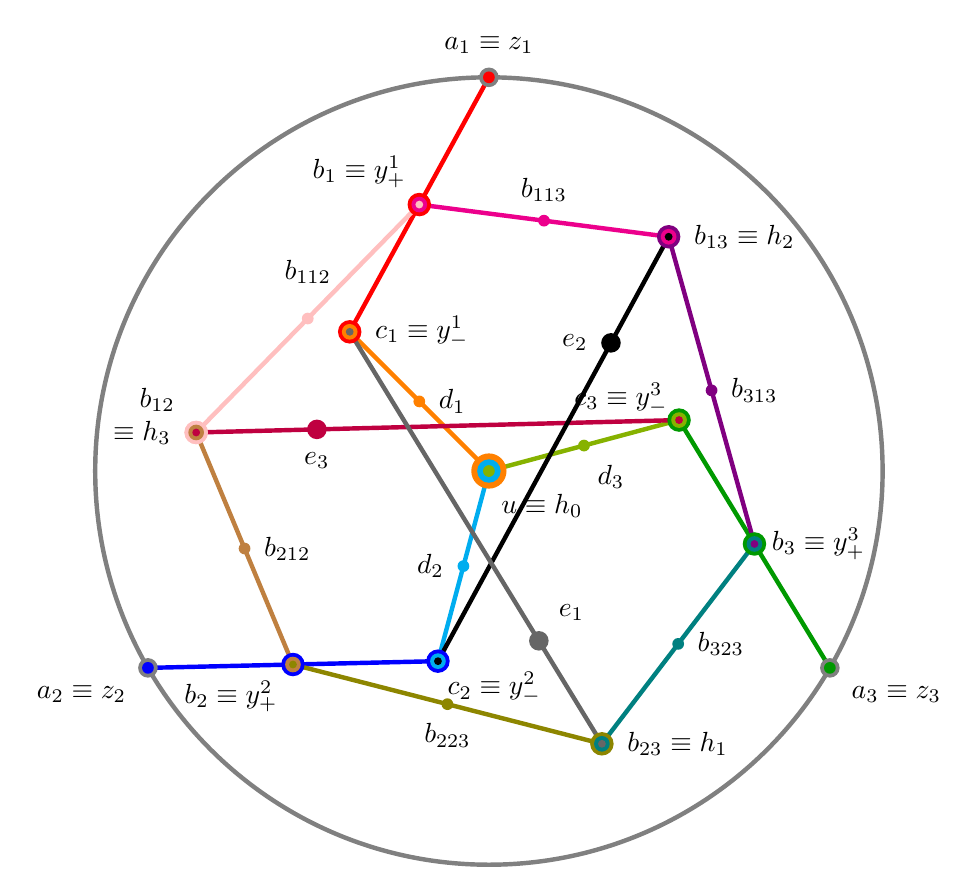
\begin{tikzpicture}[ultra thick, scale=0.5]

    % --- 1. Define all colors first for easy management ---
    \colorlet{colorCircle}{gray}
    % Colors for the three 'spokes' (a-c and c-u lines)
    \colorlet{colorAC1}{red}
    \colorlet{colorCU1}{orange}
    \colorlet{colorAC2}{blue}
    \colorlet{colorCU2}{cyan}
    \colorlet{colorAC3}{green!60!black}
    \colorlet{colorCU3}{lime!70!black}
    % Colors for the six segments of the star shape
    \colorlet{colorB1B13}{magenta}
    \colorlet{colorB13B3}{violet}
    \colorlet{colorB3B23}{teal}
    \colorlet{colorB23B2}{olive}
    \colorlet{colorB2B12}{brown}
    \colorlet{colorB12B1}{pink}
    % --- NEW: Colors for the three new connecting lines ---
    \colorlet{colorC3B12}{purple}
    \colorlet{colorC2B13}{black}   %yellow!80!
    \colorlet{colorC1B23}{black!60}


    % --- 2. Define geometric parameters ---
    \def\R{10} \def\r{5} \def\rB{7.5} \def\rD{2.5} \def\shiftangle{45}
    \def\aOneAngle{90} \def\aTwoAngle{210} \def\aThreeAngle{330}

    % --- 3. Define all coordinates without drawing the points yet ---
    \coordinate (u) at (0,0);
    \foreach \angle/\i in {\aOneAngle/1, \aTwoAngle/2, \aThreeAngle/3} {
        \coordinate (a\i) at (\angle:\R);
        \coordinate (c\i) at ({\angle+\shiftangle}:\r);
        \coordinate (d\i) at ({\angle+\shiftangle}:\rD);
    }
    \foreach \i in {1,2,3} {
        \coordinate (b\i) at ($(a\i)!0.5!(c\i)$);
    }
    \pgfmathsetmacro{\bOneAngle}{(\aOneAngle + (\aOneAngle+\shiftangle))/2}
    \pgfmathsetmacro{\bTwoAngle}{(\aTwoAngle + (\aTwoAngle+\shiftangle))/2}
    \pgfmathsetmacro{\bThreeAngle}{(\aThreeAngle + (\aThreeAngle+\shiftangle))/2}
    \pgfmathsetmacro{\bOneTwoAngle}{(\bOneAngle+\bTwoAngle)/2}
    \pgfmathsetmacro{\bTwoThreeAngle}{(\bTwoAngle+\bThreeAngle)/2}
    \pgfmathsetmacro{\bOneThreeAngle}{mod((\bThreeAngle + (\bOneAngle+360))/2, 360)}
    \coordinate (b12) at (\bOneTwoAngle:\rB);
    \coordinate (b23) at (\bTwoThreeAngle:\rB);
    \coordinate (b13) at (\bOneThreeAngle:\rB);
    \coordinate (b113) at ($(b1)!0.5!(b13)$); \coordinate (b313) at ($(b3)!0.5!(b13)$);
    \coordinate (b323) at ($(b3)!0.5!(b23)$); \coordinate (b223) at ($(b2)!0.5!(b23)$);
    \coordinate (b212) at ($(b2)!0.5!(b12)$); \coordinate (b112) at ($(b1)!0.5!(b12)$);

    % --- 4. Draw all lines with their assigned colors ---
    \draw[colorCircle] (0,0) circle (\R);
    \draw[colorAC1] (a1) -- (c1); \draw[colorCU1] (c1) -- (u);
    \draw[colorAC2] (a2) -- (c2); \draw[colorCU2] (c2) -- (u);
    \draw[colorAC3] (a3) -- (c3); \draw[colorCU3] (c3) -- (u);
    \draw[colorB1B13] (b1) -- (b13); \draw[colorB13B3] (b13) -- (b3);
    \draw[colorB3B23] (b3) -- (b23); \draw[colorB23B2] (b23) -- (b2);
    \draw[colorB2B12] (b2) -- (b12); \draw[colorB12B1] (b12) -- (b1);

    % --- NEW: Draw the three additional lines ---
    \draw[colorC3B12] (c3) -- (b12);
    \draw[colorC2B13] (c2) -- (b13);
    \draw[colorC1B23] (c1) -- (b23);

    % --- 5. Draw all points on top of the lines, with colors reflecting intersections ---
    % Points on a single line (one color)
    \node[circle, fill=colorCU1, inner sep=1.5pt, label={0:$d_1$}] at (d1) {};
    \node[circle, fill=colorCU2, inner sep=1.5pt, label={180:$d_2$}] at (d2) {};
    \node[circle, fill=colorCU3, inner sep=1.5pt, label={285:$d_3$}] at (d3) {};
    \node[circle, fill=colorB1B13, inner sep=1.5pt, label=above:$b_{113}$] at (b113) {};
    \node[circle, fill=colorB13B3, inner sep=1.5pt, label=right:$b_{313}$] at (b313) {};
    \node[circle, fill=colorB3B23, inner sep=1.5pt, label=right:$b_{323}$] at (b323) {};
    \node[circle, fill=colorB23B2, inner sep=1.5pt, label=below:$b_{223}$] at (b223) {};
    \node[circle, fill=colorB2B12, inner sep=1.5pt, label=right:$b_{212}$] at (b212) {};
    \node[circle, fill=colorB12B1, inner sep=1.5pt, label={[label distance=2mm]90:$b_{112}$}] at (b112) {};

    % Points at intersections of two lines (two colors)
    \node[circle, fill=colorCircle, inner sep=2.5pt, label={90:$a_1\equiv z_1$}] at (a1) {}; \node[circle, fill=colorAC1, inner sep=1.5pt] at (a1) {};
    \node[circle, fill=colorCircle, inner sep=2.5pt, label={210:$a_2\equiv z_2$}] at (a2) {}; \node[circle, fill=colorAC2, inner sep=1.5pt] at (a2) {};
    \node[circle, fill=colorCircle, inner sep=2.5pt, label={330:$a_3\equiv z_3$}] at (a3) {}; \node[circle, fill=colorAC3, inner sep=1.5pt] at (a3) {};

    % Points at intersections of three lines (three colors)
    % --- MODIFIED: Point u with tighter label at 275 degrees ---
    \node[circle, fill=colorCU1, inner sep=4.5pt, label={[label distance=-1mm]275:$u\equiv h_0$}] at (u) {};
    \node[circle, fill=colorCU2, inner sep=3pt] at (u) {};
    \node[circle, fill=colorCU3, inner sep=1.5pt] at (u) {};
    \node[circle, fill=colorAC1, inner sep=3pt, label={[label distance=-1mm]110:$b_1\equiv y_+^1$}] at (b1) {}; \node[circle, fill=colorB1B13, inner sep=2pt] at (b1) {}; \node[circle, fill=colorB12B1, inner sep=1pt] at (b1) {};
    \node[circle, fill=colorAC2, inner sep=3pt, label={[label distance=-1mm]230:$b_2\equiv y_+^2$}] at (b2) {}; \node[circle, fill=colorB2B12, inner sep=2pt] at (b2) {}; \node[circle, fill=colorB23B2, inner sep=1pt] at (b2) {};
    \node[circle, fill=colorAC3, inner sep=3pt, label={[label distance=-1mm]0:$b_3\equiv y_+^3$}] at (b3) {}; \node[circle, fill=colorB3B23, inner sep=2pt] at (b3) {}; \node[circle, fill=colorB13B3, inner sep=1pt] at (b3) {};

    % --- UPDATED: These points are now intersections of THREE lines ---
    \node[circle, fill=colorAC1, inner sep=3pt, label={0:$c_1\equiv y_-^1$}] at (c1) {}; \node[circle, fill=colorCU1, inner sep=2pt] at (c1) {}; \node[circle, fill=colorC1B23, inner sep=1pt] at (c1) {};
    \node[circle, fill=colorAC2, inner sep=3pt, label={[label distance=-2mm]-5:$c_2\equiv y_-^2$}] at (c2) {}; \node[circle, fill=colorCU2, inner sep=2pt] at (c2) {}; \node[circle, fill=colorC2B13, inner sep=1pt] at (c2) {};
    \node[circle, fill=colorAC3, inner sep=3pt, label={[label distance=-2.5mm]93:$c_3\equiv y_-^3$}] at (c3) {}; \node[circle, fill=colorCU3, inner sep=2pt] at (c3) {}; \node[circle, fill=colorC3B12, inner sep=1pt] at (c3) {};

    \node[circle, fill=colorB12B1, inner sep=3pt, label={above left:$b_{12}$}] at (b12) {};
    \node[circle, fill=colorB12B1, inner sep=3pt, label={left:$\equiv h_3$}] at (b12) {};
    \node[circle, fill=colorB2B12, inner sep=2pt] at (b12) {}; \node[circle, fill=colorC3B12, inner sep=1pt] at (b12) {};
    \node[circle, fill=colorB23B2, inner sep=3pt, label=right:$b_{23}\equiv h_1$] at (b23) {}; \node[circle, fill=colorB3B23, inner sep=2pt] at (b23) {}; \node[circle, fill=colorC1B23, inner sep=1pt] at (b23) {};
    \node[circle, fill=colorB13B3, inner sep=3pt, label=right:$b_{13}\equiv h_2$] at (b13) {}; \node[circle, fill=colorB1B13, inner sep=2pt] at (b13) {}; \node[circle, fill=colorC2B13, inner sep=1pt] at (b13) {};

% --- NEW: Add the three e_i points ---
    % e_1 is placed 3/4 of the way along the line from c1 to b23
    \node[circle, fill=colorC1B23, inner sep=2.5pt, label={above right:$e_1$}] (e1) at ($(c1)!0.75!(b23)$) {};

    % e_2 is placed 3/4 of the way along the line from c2 to b13
    \node[circle, fill=colorC2B13, inner sep=2.5pt, label={left:$e_2$}] (e2) at ($(c2)!0.75!(b13)$) {};

    % e_3 is placed 3/4 of the way along the line from c3 to b12
    \node[circle, fill=colorC3B12, inner sep=2.5pt, label={below:$e_3$}] (e3) at ($(c3)!0.75!(b12)$) {};

\end{tikzpicture}
}
\caption{The $25$-ray full-context completion of the original $13$-ray Yu--Oh set~\cite{Yu-2012}, drawn in the Harding and Salinas Schmeis $3$-uniform hypergraph scheme~\cite{harding2025remarksIJTP}.}
\label{fig:yohs}
\end{figure}


\begin{table*}[htbp]
\caption{\label{tab:vector_generation}
\textit{Systematic generation of the vector set for contextuality analysis.}
This table details the complete set of $225$ vectors that form the basis of our structural analysis.
A family of $25$ algebraic generation rules (rows) is applied to nine
seed vectors (columns \ensuremath{\sigma_1,\ldots,\sigma_9}).
These seeds comprise the three noncomputational MUBs in $\mathbb{C}^3$:
the Fourier basis \ensuremath{\mathcal{B}_1=\{\sigma_1,\sigma_2,\sigma_3\}},
and two related MUBs,
\ensuremath{\mathcal{B}_2=\{\sigma_4,\sigma_5,\sigma_6\}} and its complex conjugate
\ensuremath{\mathcal{B}_3=\{\sigma_7,\sigma_8,\sigma_9\}};
each yields a $69$-ray, $50$-context KS configuration.
If \ensuremath{F} is the row symbol, the entry in seed column
\ensuremath{\sigma_j} is \ensuremath{F(\sigma_j)} and receives the inventory label
\ensuremath{F_j}; for example, \ensuremath{d_1(\sigma_4)} is labelled
\ensuremath{d_{14}}.  The identity row \ensuremath{u\equiv h_0} gives
\ensuremath{u_j=\sigma_j}.
The final column counts the number of unique rays produced by each function,
highlighting the differing projective variety of the constructions.
The $165$ unique rays drawn from this set form the inventory used to identify orthogonal bases, hyperedges, or contexts.
The row symbols follow the Harding--Salinas Schmeis scheme~\cite{harding2025remarksIJTP},
with equivalences to the Yu--Oh numbering scheme~\cite{Yu-2012}.
}
\begin{ruledtabular}
\begin{tabular}{ccccccccccc}
seed&
      \multicolumn{3}{c|}{$\mathcal{B}_1$}&
      \multicolumn{3}{c|}{$\mathcal{B}_2$}&
      \multicolumn{3}{c}{$\mathcal{B}_3$}\\
\hline
rule & \ensuremath{\sigma_{1}} & \ensuremath{\sigma_{2}} & \ensuremath{\sigma_{3}} & \ensuremath{\sigma_{4}} & \ensuremath{\sigma_{5}} & \ensuremath{\sigma_{6}} & \ensuremath{\sigma_{7}} & \ensuremath{\sigma_{8}} & \ensuremath{\sigma_{9}} & \#  \\ \hline
$a_1\equiv z_1$ & $(1,0,0)$ & $(1,0,0)$ & $(1,0,0)$ & $(1,0,0)$ & $(1,0,0)$ & $(1,0,0)$ & $(1,0,0)$ & $(1,0,0)$ & $(1,0,0)$ & 1 \\
$a_2\equiv z_2$ & $(0,1,0)$ & $(0,1,0)$ & $(0,1,0)$ & $(0,1,0)$ & $(0,1,0)$ & $(0,1,0)$ & $(0,1,0)$ & $(0,1,0)$ & $(0,1,0)$ & 1 \\
$a_3\equiv z_3$ & $(0,0,1)$ & $(0,0,1)$ & $(0,0,1)$ & $(0,0,1)$ & $(0,0,1)$ & $(0,0,1)$ & $(0,0,1)$ & $(0,0,1)$ & $(0,0,1)$ & 1 \\
$u\equiv h_0$ & $(1,1,1)$ & $(1,\omega,\omega^2)$ & $(1,\omega^2,\omega)$ & $(1,\omega,\omega)$ & $(1,\omega^2,1)$ & $(1,1,\omega^2)$ & $(1,\omega^2,\omega^2)$ & $(1,\omega,1)$ & $(1,1,\omega)$ & 9 \\
$b_1\equiv y_+^1$ & $(0,1,1)$ & $(0,\omega,\omega^2)$ & $(0,\omega^2,\omega)$ & $(0,\omega,\omega)$ & $(0,\omega^2,1)$ & $(0,1,\omega^2)$ & $(0,\omega^2,\omega^2)$ & $(0,\omega,1)$ & $(0,1,\omega)$ & 3 \\
$b_2\equiv y_+^2$ & $(1,0,1)$ & $(1,0,\omega^2)$ & $(1,0,\omega)$ & $(1,0,\omega)$ & $(1,0,1)$ & $(1,0,\omega^2)$ & $(1,0,\omega^2)$ & $(1,0,1)$ & $(1,0,\omega)$ & 3 \\
$b_3\equiv y_+^3$ & $(1,1,0)$ & $(1,\omega,0)$ & $(1,\omega^2,0)$ & $(1,\omega,0)$ & $(1,\omega^2,0)$ & $(1,1,0)$ & $(1,\omega^2,0)$ & $(1,\omega,0)$ & $(1,1,0)$ & 3 \\
$c_1\equiv y_-^1$ & $(0,1,-1)$ & $(0,\omega,-\omega^2)$ & $(0,\omega^2,-\omega)$ & $(0,\omega^2,-\omega^2)$ & $(0,1,-\omega)$ & $(0,\omega,-1)$ & $(0,\omega,-\omega)$ & $(0,1,-\omega^2)$ & $(0,\omega^2,-1)$ & 3 \\
$c_2\equiv y_-^2$ & $(-1,0,1)$ & $(-\omega,0,1)$ & $(-\omega^2,0,1)$ & $(-\omega^2,0,1)$ & $(-1,0,1)$ & $(-\omega,0,1)$ & $(-\omega,0,1)$ & $(-1,0,1)$ & $(-\omega^2,0,1)$ & 3 \\
$c_3\equiv y_-^3$ & $(1,-1,0)$ & $(\omega^2,-1,0)$ & $(\omega,-1,0)$ & $(\omega^2,-1,0)$ & $(\omega,-1,0)$ & $(1,-1,0)$ & $(\omega,-1,0)$ & $(\omega^2,-1,0)$ & $(1,-1,0)$ & 3 \\
$d_1$ & $(-2,1,1)$ & $(-2,\omega,\omega^2)$ & $(-2,\omega^2,\omega)$ & $(-2,\omega,\omega)$ & $(-2,\omega^2,1)$ & $(-2,1,\omega^2)$ & $(-2,\omega^2,\omega^2)$ & $(-2,\omega,1)$ & $(-2,1,\omega)$ & 9 \\
$d_2$ & $(1,-2,1)$ & $(\omega^2,-2,\omega)$ & $(\omega,-2,\omega^2)$ & $(\omega^2,-2,1)$ & $(\omega,-2,\omega)$ & $(1,-2,\omega^2)$ & $(\omega,-2,1)$ & $(\omega^2,-2,\omega^2)$ & $(1,-2,\omega)$ & 9 \\
$d_3$ & $(1,1,-2)$ & $(\omega,\omega^2,-2)$ & $(\omega^2,\omega,-2)$ & $(\omega^2,1,-2)$ & $(1,\omega^2,-2)$ & $(\omega,\omega,-2)$ & $(\omega,1,-2)$ & $(1,\omega,-2)$ & $(\omega^2,\omega^2,-2)$ & 9 \\
$b_{12}\equiv h_3$ & $(1,1,-1)$ & $(1,\omega,-\omega^2)$ & $(1,\omega^2,-\omega)$ & $(\omega,\omega^2,-\omega^2)$ & $(\omega,1,-\omega)$ & $(\omega,\omega,-1)$ & $(\omega^2,\omega,-\omega)$ & $(\omega^2,1,-\omega^2)$ & $(\omega^2,\omega^2,-1)$ & 9 \\
$b_{13}\equiv h_2$ & $(1,-1,1)$ & $(1,-\omega,\omega^2)$ & $(1,-\omega^2,\omega)$ & $(\omega,-\omega^2,\omega^2)$ & $(\omega,-1,\omega)$ & $(\omega,-\omega,1)$ & $(\omega^2,-\omega,\omega)$ & $(\omega^2,-1,\omega^2)$ & $(\omega^2,-\omega^2,1)$ & 9 \\
$b_{23}\equiv h_1$ & $(-1,1,1)$ & $(-1,\omega,\omega^2)$ & $(-1,\omega^2,\omega)$ & $(-\omega,\omega^2,\omega^2)$ & $(-\omega,1,\omega)$ & $(-\omega,\omega,1)$ & $(-\omega^2,\omega,\omega)$ & $(-\omega^2,1,\omega^2)$ & $(-\omega^2,\omega^2,1)$ & 9 \\
$e_1$ & $(1,2,1)$ & $(\omega^2,2,\omega)$ & $(\omega,2,\omega^2)$ & $(\omega,2\omega^2,\omega^2)$ & $(1,2\omega^2,1)$ & $(\omega^2,2\omega^2,\omega)$ & $(\omega^2,2\omega,\omega)$ & $(1,2\omega,1)$ & $(\omega,2\omega,\omega^2)$ & 9 \\
$e_2$ & $(1,1,2)$ & $(\omega,\omega^2,2)$ & $(\omega^2,\omega,2)$ & $(\omega,\omega^2,2\omega^2)$ & $(\omega^2,\omega,2\omega^2)$ & $(1,1,2\omega^2)$ & $(\omega^2,\omega,2\omega)$ & $(\omega,\omega^2,2\omega)$ & $(1,1,2\omega)$ & 9 \\
$e_3$ & $(2,1,1)$ & $(2,\omega,\omega^2)$ & $(2,\omega^2,\omega)$ & $(2\omega^2,1,1)$ & $(2\omega^2,\omega,\omega^2)$ & $(2\omega^2,\omega^2,\omega)$ & $(2\omega,1,1)$ & $(2\omega,\omega^2,\omega)$ & $(2\omega,\omega,\omega^2)$ & 9 \\
$b_{112}$ & $(2,-1,1)$ & $(2,-\omega,\omega^2)$ & $(2,-\omega^2,\omega)$ & $(2,-\omega,\omega)$ & $(2,-\omega^2,1)$ & $(2,-1,\omega^2)$ & $(2,-\omega^2,\omega^2)$ & $(2,-\omega,1)$ & $(2,-1,\omega)$ & 9 \\
$b_{212}$ & $(-1,2,1)$ & $(-1,2\omega,\omega^2)$ & $(-1,2\omega^2,\omega)$ & $(-1,2\omega,\omega)$ & $(-1,2\omega^2,1)$ & $(-1,2,\omega^2)$ & $(-1,2\omega^2,\omega^2)$ & $(-1,2\omega,1)$ & $(-1,2,\omega)$ & 9 \\
$b_{113}$ & $(2,1,-1)$ & $(2,\omega,-\omega^2)$ & $(2,\omega^2,-\omega)$ & $(2,\omega,-\omega)$ & $(2,\omega^2,-1)$ & $(2,1,-\omega^2)$ & $(2,\omega^2,-\omega^2)$ & $(2,\omega,-1)$ & $(2,1,-\omega)$ & 9 \\
$b_{313}$ & $(-1,1,2)$ & $(-1,\omega,2\omega^2)$ & $(-1,\omega^2,2\omega)$ & $(-1,\omega,2\omega)$ & $(-1,\omega^2,2)$ & $(-1,1,2\omega^2)$ & $(-1,\omega^2,2\omega^2)$ & $(-1,\omega,2)$ & $(-1,1,2\omega)$ & 9 \\
$b_{223}$ & $(1,2,-1)$ & $(1,2\omega,-\omega^2)$ & $(1,2\omega^2,-\omega)$ & $(1,2\omega,-\omega)$ & $(1,2\omega^2,-1)$ & $(1,2,-\omega^2)$ & $(1,2\omega^2,-\omega^2)$ & $(1,2\omega,-1)$ & $(1,2,-\omega)$ & 9 \\
$b_{323}$ & $(1,-1,2)$ & $(1,-\omega,2\omega^2)$ & $(1,-\omega^2,2\omega)$ & $(1,-\omega,2\omega)$ & $(1,-\omega^2,2)$ & $(1,-1,2\omega^2)$ & $(1,-\omega^2,2\omega^2)$ & $(1,-\omega,2)$ & $(1,-1,2\omega)$ & 9 \\
\end{tabular}
\end{ruledtabular}
\end{table*}



\section{Global total number of $165$ non-collinear vectors in 130 orthogonal bases}

A total of $165$ unique, non-collinear vectors were identified from the analysis of the
nine seed vectors \ensuremath{\sigma_1,\ldots,\sigma_9}
in Table~\ref{tab:vector_generation}.
These vectors, which form the basis for constructing orthogonal triples, are enumerated in Table~\ref{tab:noncollinear_vectors_6col}.
The coordinate system is based on the complex third root of unity, $\omega = \mathrm{e}^{2\pi \ii{}/3}$.

This vector set is not closed with respect to the complex ``cross product''~\cite{harding2025remarksIJTP} (sometimes referred to as Hermitian cross product)
\(
u\times v =  (\overline{u_2v_3-u_3v_2},\overline{u_3v_1-u_1v_3},\overline{u_1v_2-u_2v_1})
\)
of two vectors $u=(u_1,u_2,u_3)$ and $v=(v_1,v_2,v_3)$ in $\mathbb{R}^3$ or $\mathbb{C}^3$ because, say,
$a_{11} \times d_{21} = (1,0,0) \times (1,-2,1) = -(0,1,2)$, which is not collinear with any vector of the set of globally non-collinear vectors.



\begin{table*}[htbp!]
\caption{
\rev{The complete set of $165$ projectively distinct rays, with six entries per row.  The rightmost index records the seed column in Table~\ref{tab:vector_generation}.  The $21$ rays common to all three 69-ray lineages are black.  The $48$ rays exclusive to $\mathcal{B}_1$, $\mathcal{B}_2$, and $\mathcal{B}_3$ are shown in red, green, and blue, respectively.}
}
\label{tab:noncollinear_vectors_6col}
\footnotesize % Use a smaller font to fit the content
\begin{ruledtabular}
\begin{tabular}{*{6}{c}} % 6 centered columns
{$a_{11}=(1,0,0)$} & {$a_{21}=(0,1,0)$} & {$a_{31}=(0,0,1)$} & \textcolor{red}{$u_{1}=(1,1,1)$} & \textcolor{red}{$u_{2}=(1,\omega,\omega^2)$} & \textcolor{red}{$u_{3}=(1,\omega^2,\omega)$} \\
\textcolor{green!40!black}{$u_{4}=(1,\omega,\omega)$} & \textcolor{green!40!black}{$u_{5}=(1,\omega^2,1)$} & \textcolor{green!40!black}{$u_{6}=(1,1,\omega^2)$} & \textcolor{blue}{$u_{7}=(1,\omega^2,\omega^2)$} & \textcolor{blue}{$u_{8}=(1,\omega,1)$} & \textcolor{blue}{$u_{9}=(1,1,\omega)$} \\
{$b_{11}=(0,1,1)$} & {$b_{12}=(0,\omega,\omega^2)$} & {$b_{13}=(0,\omega^2,\omega)$} & {$b_{21}=(1,0,1)$} & {$b_{22}=(1,0,\omega^2)$} & {$b_{23}=(1,0,\omega)$} \\
{$b_{31}=(1,1,0)$} & {$b_{32}=(1,\omega,0)$} & {$b_{33}=(1,\omega^2,0)$} & {$c_{11}=(0,1,-1)$} & {$c_{12}=(0,\omega,-\omega^2)$} & {$c_{13}=(0,\omega^2,-\omega)$} \\
{$c_{21}=(-1,0,1)$} & {$c_{22}=(-\omega,0,1)$} & {$c_{23}=(-\omega^2,0,1)$} & {$c_{31}=(1,-1,0)$} & {$c_{32}=(\omega^2,-1,0)$} & {$c_{33}=(\omega,-1,0)$} \\
\textcolor{red}{$d_{11}=(-2,1,1)$} & \textcolor{red}{$d_{12}=(-2,\omega,\omega^2)$} & \textcolor{red}{$d_{13}=(-2,\omega^2,\omega)$} & \textcolor{green!40!black}{$d_{14}=(-2,\omega,\omega)$} & \textcolor{green!40!black}{$d_{15}=(-2,\omega^2,1)$} & \textcolor{green!40!black}{$d_{16}=(-2,1,\omega^2)$} \\
\textcolor{blue}{$d_{17}=(-2,\omega^2,\omega^2)$} & \textcolor{blue}{$d_{18}=(-2,\omega,1)$} & \textcolor{blue}{$d_{19}=(-2,1,\omega)$} & \textcolor{red}{$d_{21}=(1,-2,1)$} & \textcolor{red}{$d_{22}=(\omega^2,-2,\omega)$} & \textcolor{red}{$d_{23}=(\omega,-2,\omega^2)$} \\
\textcolor{green!40!black}{$d_{24}=(\omega^2,-2,1)$} & \textcolor{green!40!black}{$d_{25}=(\omega,-2,\omega)$} & \textcolor{green!40!black}{$d_{26}=(1,-2,\omega^2)$} & \textcolor{blue}{$d_{27}=(\omega,-2,1)$} & \textcolor{blue}{$d_{28}=(\omega^2,-2,\omega^2)$} & \textcolor{blue}{$d_{29}=(1,-2,\omega)$} \\
\textcolor{red}{$d_{31}=(1,1,-2)$} & \textcolor{red}{$d_{32}=(\omega,\omega^2,-2)$} & \textcolor{red}{$d_{33}=(\omega^2,\omega,-2)$} & \textcolor{green!40!black}{$d_{34}=(\omega^2,1,-2)$} & \textcolor{green!40!black}{$d_{35}=(1,\omega^2,-2)$} & \textcolor{green!40!black}{$d_{36}=(\omega,\omega,-2)$} \\
\textcolor{blue}{$d_{37}=(\omega,1,-2)$} & \textcolor{blue}{$d_{38}=(1,\omega,-2)$} & \textcolor{blue}{$d_{39}=(\omega^2,\omega^2,-2)$} & \textcolor{red}{$b_{121}=(1,1,-1)$} & \textcolor{red}{$b_{122}=(1,\omega,-\omega^2)$} & \textcolor{red}{$b_{123}=(1,\omega^2,-\omega)$} \\
\textcolor{green!40!black}{$b_{124}=(\omega,\omega^2,-\omega^2)$} & \textcolor{green!40!black}{$b_{125}=(\omega,1,-\omega)$} & \textcolor{green!40!black}{$b_{126}=(\omega,\omega,-1)$} & \textcolor{blue}{$b_{127}=(\omega^2,\omega,-\omega)$} & \textcolor{blue}{$b_{128}=(\omega^2,1,-\omega^2)$} & \textcolor{blue}{$b_{129}=(\omega^2,\omega^2,-1)$} \\
\textcolor{red}{$b_{131}=(1,-1,1)$} & \textcolor{red}{$b_{132}=(1,-\omega,\omega^2)$} & \textcolor{red}{$b_{133}=(1,-\omega^2,\omega)$} & \textcolor{green!40!black}{$b_{134}=(\omega,-\omega^2,\omega^2)$} & \textcolor{green!40!black}{$b_{135}=(\omega,-1,\omega)$} & \textcolor{green!40!black}{$b_{136}=(\omega,-\omega,1)$} \\
\textcolor{blue}{$b_{137}=(\omega^2,-\omega,\omega)$} & \textcolor{blue}{$b_{138}=(\omega^2,-1,\omega^2)$} & \textcolor{blue}{$b_{139}=(\omega^2,-\omega^2,1)$} & \textcolor{red}{$b_{231}=(-1,1,1)$} & \textcolor{red}{$b_{232}=(-1,\omega,\omega^2)$} & \textcolor{red}{$b_{233}=(-1,\omega^2,\omega)$} \\
\textcolor{green!40!black}{$b_{234}=(-\omega,\omega^2,\omega^2)$} & \textcolor{green!40!black}{$b_{235}=(-\omega,1,\omega)$} & \textcolor{green!40!black}{$b_{236}=(-\omega,\omega,1)$} & \textcolor{blue}{$b_{237}=(-\omega^2,\omega,\omega)$} & \textcolor{blue}{$b_{238}=(-\omega^2,1,\omega^2)$} & \textcolor{blue}{$b_{239}=(-\omega^2,\omega^2,1)$} \\
\textcolor{red}{$e_{11}=(1,2,1)$} & \textcolor{red}{$e_{12}=(\omega^2,2,\omega)$} & \textcolor{red}{$e_{13}=(\omega,2,\omega^2)$} & \textcolor{green!40!black}{$e_{14}=(\omega,2\omega^2,\omega^2)$} & \textcolor{green!40!black}{$e_{15}=(1,2\omega^2,1)$} & \textcolor{green!40!black}{$e_{16}=(\omega^2,2\omega^2,\omega)$} \\
\textcolor{blue}{$e_{17}=(\omega^2,2\omega,\omega)$} & \textcolor{blue}{$e_{18}=(1,2\omega,1)$} & \textcolor{blue}{$e_{19}=(\omega,2\omega,\omega^2)$} & \textcolor{red}{$e_{21}=(1,1,2)$} & \textcolor{red}{$e_{22}=(\omega,\omega^2,2)$} & \textcolor{red}{$e_{23}=(\omega^2,\omega,2)$} \\
\textcolor{green!40!black}{$e_{24}=(\omega,\omega^2,2\omega^2)$} & \textcolor{green!40!black}{$e_{25}=(\omega^2,\omega,2\omega^2)$} & \textcolor{green!40!black}{$e_{26}=(1,1,2\omega^2)$} & \textcolor{blue}{$e_{27}=(\omega^2,\omega,2\omega)$} & \textcolor{blue}{$e_{28}=(\omega,\omega^2,2\omega)$} & \textcolor{blue}{$e_{29}=(1,1,2\omega)$} \\
\textcolor{red}{$e_{31}=(2,1,1)$} & \textcolor{red}{$e_{32}=(2,\omega,\omega^2)$} & \textcolor{red}{$e_{33}=(2,\omega^2,\omega)$} & \textcolor{green!40!black}{$e_{34}=(2\omega^2,1,1)$} & \textcolor{green!40!black}{$e_{35}=(2\omega^2,\omega,\omega^2)$} & \textcolor{green!40!black}{$e_{36}=(2\omega^2,\omega^2,\omega)$} \\
\textcolor{blue}{$e_{37}=(2\omega,1,1)$} & \textcolor{blue}{$e_{38}=(2\omega,\omega^2,\omega)$} & \textcolor{blue}{$e_{39}=(2\omega,\omega,\omega^2)$} & \textcolor{red}{$b_{1121}=(2,-1,1)$} & \textcolor{red}{$b_{1122}=(2,-\omega,\omega^2)$} & \textcolor{red}{$b_{1123}=(2,-\omega^2,\omega)$} \\
\textcolor{green!40!black}{$b_{1124}=(2,-\omega,\omega)$} & \textcolor{green!40!black}{$b_{1125}=(2,-\omega^2,1)$} & \textcolor{green!40!black}{$b_{1126}=(2,-1,\omega^2)$} & \textcolor{blue}{$b_{1127}=(2,-\omega^2,\omega^2)$} & \textcolor{blue}{$b_{1128}=(2,-\omega,1)$} & \textcolor{blue}{$b_{1129}=(2,-1,\omega)$} \\
\textcolor{red}{$b_{2121}=(-1,2,1)$} & \textcolor{red}{$b_{2122}=(-1,2\omega,\omega^2)$} & \textcolor{red}{$b_{2123}=(-1,2\omega^2,\omega)$} & \textcolor{green!40!black}{$b_{2124}=(-1,2\omega,\omega)$} & \textcolor{green!40!black}{$b_{2125}=(-1,2\omega^2,1)$} & \textcolor{green!40!black}{$b_{2126}=(-1,2,\omega^2)$} \\
\textcolor{blue}{$b_{2127}=(-1,2\omega^2,\omega^2)$} & \textcolor{blue}{$b_{2128}=(-1,2\omega,1)$} & \textcolor{blue}{$b_{2129}=(-1,2,\omega)$} & \textcolor{red}{$b_{1131}=(2,1,-1)$} & \textcolor{red}{$b_{1132}=(2,\omega,-\omega^2)$} & \textcolor{red}{$b_{1133}=(2,\omega^2,-\omega)$} \\
\textcolor{green!40!black}{$b_{1134}=(2,\omega,-\omega)$} & \textcolor{green!40!black}{$b_{1135}=(2,\omega^2,-1)$} & \textcolor{green!40!black}{$b_{1136}=(2,1,-\omega^2)$} & \textcolor{blue}{$b_{1137}=(2,\omega^2,-\omega^2)$} & \textcolor{blue}{$b_{1138}=(2,\omega,-1)$} & \textcolor{blue}{$b_{1139}=(2,1,-\omega)$} \\
\textcolor{red}{$b_{3131}=(-1,1,2)$} & \textcolor{red}{$b_{3132}=(-1,\omega,2\omega^2)$} & \textcolor{red}{$b_{3133}=(-1,\omega^2,2\omega)$} & \textcolor{green!40!black}{$b_{3134}=(-1,\omega,2\omega)$} & \textcolor{green!40!black}{$b_{3135}=(-1,\omega^2,2)$} & \textcolor{green!40!black}{$b_{3136}=(-1,1,2\omega^2)$} \\
\textcolor{blue}{$b_{3137}=(-1,\omega^2,2\omega^2)$} & \textcolor{blue}{$b_{3138}=(-1,\omega,2)$} & \textcolor{blue}{$b_{3139}=(-1,1,2\omega)$} & \textcolor{red}{$b_{2231}=(1,2,-1)$} & \textcolor{red}{$b_{2232}=(1,2\omega,-\omega^2)$} & \textcolor{red}{$b_{2233}=(1,2\omega^2,-\omega)$} \\
\textcolor{green!40!black}{$b_{2234}=(1,2\omega,-\omega)$} & \textcolor{green!40!black}{$b_{2235}=(1,2\omega^2,-1)$} & \textcolor{green!40!black}{$b_{2236}=(1,2,-\omega^2)$} & \textcolor{blue}{$b_{2237}=(1,2\omega^2,-\omega^2)$} & \textcolor{blue}{$b_{2238}=(1,2\omega,-1)$} & \textcolor{blue}{$b_{2239}=(1,2,-\omega)$} \\
\textcolor{red}{$b_{3231}=(1,-1,2)$} & \textcolor{red}{$b_{3232}=(1,-\omega,2\omega^2)$} & \textcolor{red}{$b_{3233}=(1,-\omega^2,2\omega)$} & \textcolor{green!40!black}{$b_{3234}=(1,-\omega,2\omega)$} & \textcolor{green!40!black}{$b_{3235}=(1,-\omega^2,2)$} & \textcolor{green!40!black}{$b_{3236}=(1,-1,2\omega^2)$} \\
\textcolor{blue}{$b_{3237}=(1,-\omega^2,2\omega^2)$} & \textcolor{blue}{$b_{3238}=(1,-\omega,2)$} & \textcolor{blue}{$b_{3239}=(1,-1,2\omega)$} & & & \\
\end{tabular}
\end{ruledtabular}
\end{table*}




\begin{table*}[htbp!]
\caption{
\rev{The complete list of $130$ orthogonal bases supported by the $165$ rays.
The invariant provenance counts are stated in Proposition~\ref{prop:provenance}.}
}
\label{tab:orthogonal_bases}
\begin{ruledtabular}
\begin{tabular}{ccccccc} %

% --- Table Content (6 bases per row) ---
{\{$a_{11}$, $a_{21}$, $a_{31}$\}} & {\{$a_{11}$, $b_{11}$, $c_{11}$\}} & {\{$a_{11}$, $b_{12}$, $c_{12}$\}} & {\{$a_{11}$, $b_{13}$, $c_{13}$\}} & {\{$a_{21}$, $b_{21}$, $c_{21}$\}} & {\{$a_{21}$, $b_{22}$, $c_{22}$\}} \\
{\{$a_{21}$, $b_{23}$, $c_{23}$\}} & {\{$a_{31}$, $b_{31}$, $c_{31}$\}} & {\{$a_{31}$, $b_{32}$, $c_{32}$\}} & {\{$a_{31}$, $b_{33}$, $c_{33}$\}} & \{$u_{1}$, $u_{2}$, $u_{3}$\} & \{$u_{1}$, $c_{11}$, $d_{11}$\} \\
\{$u_{1}$, $c_{21}$, $d_{21}$\} & \{$u_{1}$, $c_{31}$, $d_{31}$\} & \{$u_{2}$, $c_{12}$, $d_{12}$\} & \{$u_{2}$, $c_{22}$, $d_{22}$\} & \{$u_{2}$, $c_{32}$, $d_{32}$\} & \{$u_{3}$, $c_{13}$, $d_{13}$\} \\
\{$u_{3}$, $c_{23}$, $d_{23}$\} & \{$u_{3}$, $c_{33}$, $d_{33}$\} & \{$u_{4}$, $u_{5}$, $u_{6}$\} & \{$u_{4}$, $c_{11}$, $d_{14}$\} & \{$u_{4}$, $c_{23}$, $d_{24}$\} & \{$u_{4}$, $c_{32}$, $d_{34}$\} \\
\{$u_{5}$, $c_{12}$, $d_{15}$\} & \{$u_{5}$, $c_{21}$, $d_{25}$\} & \{$u_{5}$, $c_{33}$, $d_{35}$\} & \{$u_{6}$, $c_{13}$, $d_{16}$\} & \{$u_{6}$, $c_{22}$, $d_{26}$\} & \{$u_{6}$, $c_{31}$, $d_{36}$\} \\
\{$u_{7}$, $u_{8}$, $u_{9}$\} & \{$u_{7}$, $c_{11}$, $d_{17}$\} & \{$u_{7}$, $c_{22}$, $d_{27}$\} & \{$u_{7}$, $c_{33}$, $d_{37}$\} & \{$u_{8}$, $c_{13}$, $d_{18}$\} & \{$u_{8}$, $c_{21}$, $d_{28}$\} \\
\{$u_{8}$, $c_{32}$, $d_{38}$\} & \{$u_{9}$, $c_{12}$, $d_{19}$\} & \{$u_{9}$, $c_{23}$, $d_{29}$\} & \{$u_{9}$, $c_{31}$, $d_{39}$\} & \{$b_{11}$, $b_{121}$, $b_{1121}$\} & \{$b_{11}$, $b_{124}$, $b_{1124}$\} \\
\{$b_{11}$, $b_{127}$, $b_{1127}$\} & \{$b_{11}$, $b_{131}$, $b_{1131}$\} & \{$b_{11}$, $b_{134}$, $b_{1134}$\} & \{$b_{11}$, $b_{137}$, $b_{1137}$\} & \{$b_{12}$, $b_{122}$, $b_{1122}$\} & \{$b_{12}$, $b_{125}$, $b_{1125}$\} \\
\{$b_{12}$, $b_{129}$, $b_{1129}$\} & \{$b_{12}$, $b_{132}$, $b_{1132}$\} & \{$b_{12}$, $b_{135}$, $b_{1135}$\} & \{$b_{12}$, $b_{139}$, $b_{1139}$\} & \{$b_{13}$, $b_{123}$, $b_{1123}$\} & \{$b_{13}$, $b_{126}$, $b_{1126}$\} \\
\{$b_{13}$, $b_{128}$, $b_{1128}$\} & \{$b_{13}$, $b_{133}$, $b_{1133}$\} & \{$b_{13}$, $b_{136}$, $b_{1136}$\} & \{$b_{13}$, $b_{138}$, $b_{1138}$\} & \{$b_{21}$, $b_{121}$, $b_{2121}$\} & \{$b_{21}$, $b_{125}$, $b_{2125}$\} \\
\{$b_{21}$, $b_{128}$, $b_{2128}$\} & \{$b_{21}$, $b_{231}$, $b_{2231}$\} & \{$b_{21}$, $b_{235}$, $b_{2235}$\} & \{$b_{21}$, $b_{238}$, $b_{2238}$\} & \{$b_{22}$, $b_{122}$, $b_{2122}$\} & \{$b_{22}$, $b_{126}$, $b_{2126}$\} \\
\{$b_{22}$, $b_{127}$, $b_{2127}$\} & \{$b_{22}$, $b_{232}$, $b_{2232}$\} & \{$b_{22}$, $b_{236}$, $b_{2236}$\} & \{$b_{22}$, $b_{237}$, $b_{2237}$\} & \{$b_{23}$, $b_{123}$, $b_{2123}$\} & \{$b_{23}$, $b_{124}$, $b_{2124}$\} \\
\{$b_{23}$, $b_{129}$, $b_{2129}$\} & \{$b_{23}$, $b_{233}$, $b_{2233}$\} & \{$b_{23}$, $b_{234}$, $b_{2234}$\} & \{$b_{23}$, $b_{239}$, $b_{2239}$\} & \{$b_{31}$, $b_{131}$, $b_{3131}$\} & \{$b_{31}$, $b_{136}$, $b_{3136}$\} \\
\{$b_{31}$, $b_{139}$, $b_{3139}$\} & \{$b_{31}$, $b_{231}$, $b_{3231}$\} & \{$b_{31}$, $b_{236}$, $b_{3236}$\} & \{$b_{31}$, $b_{239}$, $b_{3239}$\} & \{$b_{32}$, $b_{132}$, $b_{3132}$\} & \{$b_{32}$, $b_{134}$, $b_{3134}$\} \\
\{$b_{32}$, $b_{138}$, $b_{3138}$\} & \{$b_{32}$, $b_{232}$, $b_{3232}$\} & \{$b_{32}$, $b_{234}$, $b_{3234}$\} & \{$b_{32}$, $b_{238}$, $b_{3238}$\} & \{$b_{33}$, $b_{133}$, $b_{3133}$\} & \{$b_{33}$, $b_{135}$, $b_{3135}$\} \\
\{$b_{33}$, $b_{137}$, $b_{3137}$\} & \{$b_{33}$, $b_{233}$, $b_{3233}$\} & \{$b_{33}$, $b_{235}$, $b_{3235}$\} & \{$b_{33}$, $b_{237}$, $b_{3237}$\} & \{$c_{11}$, $b_{231}$, $e_{31}$\} & \{$c_{11}$, $b_{234}$, $e_{34}$\} \\
\{$c_{11}$, $b_{237}$, $e_{37}$\} & \{$c_{12}$, $b_{232}$, $e_{32}$\} & \{$c_{12}$, $b_{235}$, $e_{35}$\} & \{$c_{12}$, $b_{239}$, $e_{39}$\} & \{$c_{13}$, $b_{233}$, $e_{33}$\} & \{$c_{13}$, $b_{236}$, $e_{36}$\} \\
\{$c_{13}$, $b_{238}$, $e_{38}$\} & \{$c_{21}$, $b_{131}$, $e_{11}$\} & \{$c_{21}$, $b_{135}$, $e_{15}$\} & \{$c_{21}$, $b_{138}$, $e_{18}$\} & \{$c_{22}$, $b_{132}$, $e_{12}$\} & \{$c_{22}$, $b_{136}$, $e_{16}$\} \\
\{$c_{22}$, $b_{137}$, $e_{17}$\} & \{$c_{23}$, $b_{133}$, $e_{13}$\} & \{$c_{23}$, $b_{134}$, $e_{14}$\} & \{$c_{23}$, $b_{139}$, $e_{19}$\} & \{$c_{31}$, $b_{121}$, $e_{21}$\} & \{$c_{31}$, $b_{126}$, $e_{26}$\} \\
\{$c_{31}$, $b_{129}$, $e_{29}$\} & \{$c_{32}$, $b_{122}$, $e_{22}$\} & \{$c_{32}$, $b_{124}$, $e_{24}$\} & \{$c_{32}$, $b_{128}$, $e_{28}$\} & \{$c_{33}$, $b_{123}$, $e_{23}$\} & \{$c_{33}$, $b_{125}$, $e_{25}$\} \\
\{$c_{33}$, $b_{127}$, $e_{27}$\} & \{$b_{121}$, $b_{122}$, $b_{123}$\} & \{$b_{124}$, $b_{125}$, $b_{126}$\} & \{$b_{127}$, $b_{128}$, $b_{129}$\} & \{$b_{131}$, $b_{132}$, $b_{133}$\} & \{$b_{134}$, $b_{135}$, $b_{136}$\} \\
\{$b_{137}$, $b_{138}$, $b_{139}$\} & \{$b_{231}$, $b_{232}$, $b_{233}$\} & \{$b_{234}$, $b_{235}$, $b_{236}$\} & \{$b_{237}$, $b_{238}$, $b_{239}$\} & & \\
\end{tabular}
\end{ruledtabular}
\end{table*}

\begin{revision}
\subsection{Symmetric provenance decomposition}

For $r=1,2,3$, let $\mathcal{S}_r$ be the projective ray set generated from the three seeds in $\mathcal{B}_r$, and let $\mathcal{E}_r$ be its set of orthogonal triples.

\begin{proposition}[Ray and context inventory]
\label{prop:provenance}
The generated families satisfy
\[
|\mathcal{S}_r|=69,\qquad
|\mathcal{S}_1\cap\mathcal{S}_2\cap\mathcal{S}_3|=21,
\qquad |\mathcal{S}_r\setminus(\mathcal{S}_s\cup\mathcal{S}_t)|=48,
\]
where $\{r,s,t\}=\{1,2,3\}$, and no ray belongs to exactly two lineages.  Their union has $165$
rays.  Likewise, each $\mathcal{E}_r$ contains $50$ contexts, $10$ contexts are common to all three lineages, and each lineage contributes $40$ further contexts.  The union therefore contains $10+3\cdot40=130$ contexts.  Exactly four contexts in each lineage consist entirely of lineage-exclusive rays.
\end{proposition}

\begin{proof}
Each nonzero generated vector is divided by its first nonzero coordinate to obtain a canonical projective representative.  Equality is then decided using $1+\omega+\omega^2=0$.  This gives $69$ representatives per lineage and the overlap counts above.  Pairwise Hermitian inner products are evaluated exactly in $\mathbb{Q}(\omega)$; triangles in the resulting orthogonality graph are precisely the contexts.  The exhaustive search gives $50$ contexts per lineage and $130$ in the union.  Finally, direct enumeration of maps $s:V\to\{0,1\}$ with one $1$ per context gives no two-valued state for any of the three $69$-ray, $50$-context lineages.
\end{proof}

The symmetric provenance statement depends on the complete sets of generating lineages and is independent of the display labels assigned to the rays.
\end{revision}


%\onecolumngrid




\section{Higher-dimensional forcing gadgets}
\label{2025-hdfg}

\begin{revision}
In $\mathcal{P}(\mathbb{C}^3)$, two independent rays determine a unique orthogonal ray.  For $D\geq4$, their orthogonal complement has dimension $D-2$, so additional connector contexts are required to obtain a rigid finite construction.

\begin{definition}[Unbiased vector]
\label{def:unbiased}
A normalized vector $u$ is maximally unbiased relative to an orthonormal basis $\mathcal{B}$ if
\[
|\langle e_j,u\rangle|^2=1/D\quad (j=1,\ldots,D).
\]
For $u=(x_1,\ldots,x_D)$ in the computational basis, this is equivalent to \ensuremath{|x_1|=\cdots=|x_D|}.
\end{definition}

The $D=4$ and $D=5$ constructions have three logically separate parts: (i) a scaffold of coordinate-supported minors, (ii) connector rays whose orthogonality to the center gives equations in $|x_j|^2$, and (iii) completion vectors that turn the required orthogonal pairs into full contexts.  The propositions below state the forcing constraints; coordinate inventories and exact enumeration checks are given afterward.
\end{revision}

\subsection{Notation and conventions}
Fix an unknown center vector $u = (x_1,\dots,x_D) \in \mathbb{C}^D$ with $x_j \ne 0$ for all $j$, and use the standard Hermitian inner product
\[
\langle v,w\rangle = \sum_m \overline{v_m}\, w_m.
\]
We use vectors to represent the one-dimensional subspaces they span and freely scale them when forming blocks,
with the understanding that they must be normalized to form a literal orthonormal basis.

\subsection{An explicit gadget for $D=4$}

%\subsubsection{Rim (computational basis).}
\rev{First, take the computational (Cartesian) basis}
\begin{align*}
e_1&=(1,0,0,0), &
e_2 =(0,1,0,0),\\
e_3&=(0,0,1,0), &
e_4 =(0,0,0,1),
\end{align*}
\rev{and place the context $\mathcal{B}_{\mathrm{comp}}=\{e_1,e_2,e_3,e_4\}$ on the rim of Fig.~\ref{fig:peres}(a).}

%\subsubsection{Pair minors (Levi-Civita contraction).}
In the second construction stage define, for each unordered pair $\{i,j\}\subset\{1,2,3,4\}$, pair minors from a Levi-Civita contraction:
\begin{align*}
v_{12} &= (0,0,\overline{x_4},-\overline{x_3}), &
v_{13}  = (0,-\overline{x_4},0,\overline{x_2}), \\
v_{14} &= (0,\overline{x_3},-\overline{x_2},0), &
v_{23}  = (\overline{x_4},0,0,-\overline{x_1}), \\
v_{24} &= (-\overline{x_3},0,\overline{x_1},0), &
v_{34}  = (\overline{x_2},-\overline{x_1},0,0).
\end{align*}
Each $v_{ij}$ vanishes in coordinates $i,j$ and satisfies $\langle v_{ij},u\rangle=0$ by direct cancellation.

%\subsubsection{Complementary atoms and pair blocks.}
In the third step, choose a vector $w_{ij}$ with the same support as $v_{ij}$ and orthogonal to it, that is, $\langle v_{ij},w_{ij}\rangle=0$:
\begin{align*}
w_{12}&=(0,0,x_3,x_4), &
w_{13} =(0,x_2,0,x_4), \\
w_{14}&=(0,x_2,x_3,0), &
w_{23} =(x_1,0,0,x_4), \\
w_{24}&=(x_1,0,x_3,0), &
w_{34} =(x_1,x_2,0,0).
\end{align*}
\rev{For each of the $\binom{4}{2}=6$ pairs $\{i,j\}$, the set}
\[
\mathcal{B}_{ij}=\{e_i, e_j, v_{ij}, w_{ij}\}
\]
is an orthogonal basis (block, context).

In a fourth step, define three connector vectors
\begin{align*}
v_{1234}&=(x_1,x_2,-x_3,-x_4),\\
v_{1324}&=(x_1,-x_2,x_3,-x_4),\\
v_{1423}&=(x_1,-x_2,-x_3,x_4).
\end{align*}
\begin{revision}
Whenever $u$ is orthogonal to one of these connector vectors, the two-dimensional complement of their span supplies completion rays $h_1,h_2$.  Thus the three connector contexts may be written
\begin{align*}
\mathcal{C}_{(a)}&=\{u,v_{1234},h^{(a)}_1,h^{(a)}_2\},&
\mathcal{C}_{(b)}&=\{u,v_{1324},h^{(b)}_1,h^{(b)}_2\},\\
\mathcal{C}_{(c)}&=\{u,v_{1423},h^{(c)}_1,h^{(c)}_2\}.
\end{align*}

\begin{proposition}[$D=4$ forcing constraint]
\label{prop:D4forcing}
Membership of $u$ and the three connector rays in the contexts above forces $u$ to be maximally unbiased relative to $\mathcal{B}_{\mathrm{comp}}$.
\end{proposition}

\begin{proof}
The three required inner products vanish exactly when
\begin{align}
|x_1|^2+|x_2|^2&=|x_3|^2+|x_4|^2, \label{eq:D4a}\\
|x_1|^2+|x_3|^2&=|x_2|^2+|x_4|^2, \label{eq:D4b}\\
|x_1|^2+|x_4|^2&=|x_2|^2+|x_3|^2. \label{eq:D4c}
\end{align}
Subtracting pairs of equations gives $|x_2|^2=|x_3|^2=|x_4|^2$; substitution gives $|x_1|^2=|x_2|^2$.  Since the moduli are nonnegative, \ensuremath{|x_1|=|x_2|=|x_3|=|x_4|}.  After normalization, every squared modulus is $1/4$.
\end{proof}

\subsubsection{Automatic and equality-induced contexts}
Orthogonalities due only to disjoint support, such as $v_{12}\perp v_{34}$, do not constrain $u$.  For the concrete 20-ray representation with $u=(1,1,1,1)$, the computational context, six pair contexts, and three connector contexts give 10 imposed contexts.  An exhaustive orthogonality search finds exactly seven further contexts.  Three follow from disjoint support:
\begin{align*}
\mathcal{B}_{1234}&=\{v_{12},w_{12},v_{34},w_{34}\},\\
\mathcal{B}_{1324}&=\{v_{13},w_{13},v_{24},w_{24}\},\\
\mathcal{B}_{1423}&=\{v_{14},w_{14},v_{23},w_{23}\}.
\end{align*}
The remaining four use the equal-modulus relations from Proposition~\ref{prop:D4forcing}:
\begin{align*}
\mathcal{C}_0&=\{u,v_{1234},v_{1324},v_{1423}\},\\
\mathcal{E}_1&=\{w_{12},w_{34},v_{1324},v_{1423}\},\\
\mathcal{E}_2&=\{w_{13},w_{24},v_{1234},v_{1423}\},\\
\mathcal{E}_3&=\{w_{14},w_{23},v_{1234},v_{1324}\}.
\end{align*}
Hence the complete orthogonality hypergraph of the concrete $20$-ray set has $17$ contexts, not $13$.  Exact enumeration gives $16$ two-valued states, and these states separate every pair of rays; the complete $20$-ray hypergraph is therefore not a KS configuration.
\end{revision}

\begin{figure*}[ht]
\centering
\begin{tabular}{ccc}
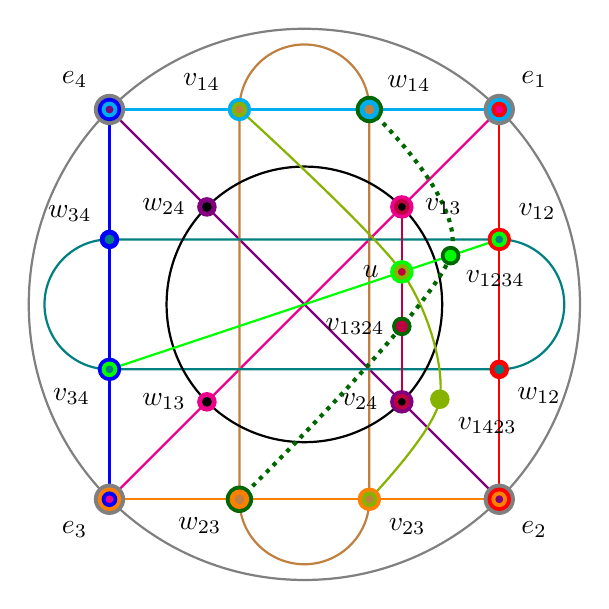
\begin{tikzpicture}[thick, scale=0.35]
    % --- Add necessary TikZ libraries ---
    \usetikzlibrary{decorations.markings, intersections}

    % --- 1. Define all colors ---
    \colorlet{colorCircle}{gray}
    \colorlet{colorE1E2}{red} \colorlet{colorE2E3}{orange}
    \colorlet{colorE3E4}{blue} \colorlet{colorE4E1}{cyan}
    \colorlet{colorV12V34}{green} \colorlet{colorV23V41}{lime!70!black}
    \colorlet{colorCurve13}{magenta} \colorlet{colorCurve24}{violet}
    \colorlet{colorV13V24}{purple}
    \colorlet{colorHiddenA}{brown} \colorlet{colorHiddenB}{teal}
    \colorlet{colorEllipse}{black}   %yellow!80!
    \colorlet{darkgreen}{green!40!black}

    % --- 2. Define geometric parameters ---
    \def\R{10} \def\bendangle{30}

    % --- 3. Define ALL coordinates first, without drawing ---
    \foreach \angle/\i in {45/1, 315/2, 225/3, 135/4} { \coordinate (e\i) at (\angle:\R); }
    \foreach \i/\j in {1/2, 2/3, 3/4, 4/1} {
        \coordinate (v\i\j) at ($(e\i)!1/3!(e\j)$);
        \coordinate (w\i\j) at ($(e\i)!2/3!(e\j)$);
    }
    \coordinate (v13) at ($(e1)!1/4!(e3)$);
    \coordinate (v24) at ($(e2)!1/4!(e4)$);
    \coordinate (w13) at ($(e1)!3/4!(e3)$);
    \coordinate (w24) at ($(e2)!3/4!(e4)$);

    % --- CHANGE: Define u at 0.6 of the distance along the curved green path from v34.
    % \path[
    %     postaction={decorate, decoration={
    %         markings,
    %         mark=at position 0.6 with {\coordinate (u) at (0,0);}
    %     }}
    % ] (v34) to[bend right=\bendangle/2] (v12);
    \path[name path=curve-v12-v34] (v34) -- (v12);
    \path[name path=curve-v13-v24] (v13) -- (v24);
    \path[name intersections={of=curve-v12-v34 and curve-v13-v24, by=u}];

    % All coordinates that depend on u will now be automatically updated.
    \coordinate (g12) at ($(u)!0.5!(v12)$);
    \coordinate (g13) at ($(u)!0.5!(v13)$);
    \coordinate (g23) at (325:\R*.6); % This is the coordinate for node v1423
    % \coordinate (g23) at ($(u)!0.8!(v41)$); % This is the coordinate for node v1423
    \path (e1) (v13) (w13) (e3);
    \path (e2) (v24) (w24) (e4);

    % --- 4. Draw all lines and curves ---
    \draw[colorCircle] (0,0) circle (\R);
    \draw[colorE1E2] (e1) -- (e2); \draw[colorE2E3] (e2) -- (e3);
    \draw[colorE3E4] (e3) -- (e4); \draw[colorE4E1] (e4) -- (e1);
    \draw[colorCurve13] (e1) -- (e3);
    \draw[colorCurve24] (e2) -- (e4);

    \draw[colorHiddenA] (v41) -- (w23); \draw[colorHiddenA] (w41) -- (v23);
    \draw[colorHiddenB] (v12) -- (w34); \draw[colorHiddenB] (w12) -- (v34);
    \draw[colorEllipse] (0,0) circle (\R/2);
    \draw[colorHiddenA] let \p1=($(w41)-(v41)$), \n1={atan2(\y1,\x1)}, \n2={veclen(\x1,\y1)/2} in (w41) arc (\n1:\n1+180:\n2);
    \draw[colorHiddenA] let \p1=($(w23)-(v23)$), \n1={atan2(\y1,\x1)}, \n2={veclen(\x1,\y1)/2} in (w23) arc (\n1:\n1+180:\n2);
    \draw[colorHiddenB] let \p1=($(w12)-(v12)$), \n1={atan2(\y1,\x1)}, \n2={veclen(\x1,\y1)/2} in (w12) arc (\n1:\n1+180:\n2);
    \draw[colorHiddenB] let \p1=($(w34)-(v34)$), \n1={atan2(\y1,\x1)}, \n2={veclen(\x1,\y1)/2} in (w34) arc (\n1:\n1+180:\n2);

    % Draw the green curve.
    % \draw[colorV12V34] (v34) to[bend right=\bendangle/2] (v12);
    \draw[colorV12V34] (v34) -- (v12);

    % The lime!70!black curve automatically adjusts to the new position of u.
    \draw[colorV23V41] plot[smooth, tension=0.5] coordinates {(v41) (u) (g23) (v23)};

    % Dotted green curve adjusts because its shape depends on g12, which depends on u.
    % \draw[darkgreen, dotted, line width=1.5pt,
    %     postaction={decorate, decoration={
    %         markings,
    %         mark=at position 0.15 with {\coordinate (v1324) at (0,0);}
    %     }}
    % ] plot[smooth cycle, tension=0.5] coordinates {(w41) (w23) (g12)};
    \draw[darkgreen, dotted, line width=1.5pt] plot[smooth, tension=0.5] coordinates {(w41) (g12) (w23)};
    \path[name path=curve-w41-w23] plot[smooth, tension=0.5] coordinates {(w41) (g12) (w23)};
    \path[name intersections={of=curve-w41-w23 and curve-v13-v24, by=v1324}];
    % The purple curve automatically adjusts to the new position of u.
    % \draw[colorV13V24] plot[smooth, tension=0.8] coordinates {(v24) %(v1324)
    % (u) (v13)};
    \draw[colorV13V24] (v24) -- (v13);
    % --- 5. Draw all points on TOP ---
    \node[circle, fill=darkgreen, inner sep=2.5pt] at (v1324) {};
    \node[circle, fill=colorV13V24, inner sep=1.5pt, label={left:$v_{1324}$}] at (v1324) {};

    \node[circle, fill=darkgreen, inner sep=2.5pt] at (g12) {};
    \node[circle, fill=colorV12V34, inner sep=1.5pt, label={below right:$v_{1234}$}] at (g12) {};
    \node[circle, fill=colorV23V41, inner sep=2.5pt, label={below right:$v_{1423}$}] at (g23) {};
    \node[circle, fill=colorV12V34, inner sep=3pt, label={left:$u$}] at (u) {}; \node[circle, fill=colorV23V41, inner sep=2pt] at (u) {}; \node[circle, fill=colorV13V24, inner sep=1pt] at (u) {};
    \node[circle, fill=colorCurve13, inner sep=3pt, label={right:$v_{13}$}] at (v13) {}; \node[circle, fill=colorV13V24, inner sep=2pt] at (v13) {}; \node[circle, fill=colorEllipse, inner sep=1pt] at (v13) {};
    \node[circle, fill=colorCurve24, inner sep=3pt, label={left:$v_{24}$}] at (v24) {}; \node[circle, fill=colorV13V24, inner sep=2pt] at (v24) {}; \node[circle, fill=colorEllipse, inner sep=1pt] at (v24) {};
    \node[circle, fill=colorCurve13, inner sep=2.5pt, label={left:$w_{13}$}] at (w13) {}; \node[circle, fill=colorEllipse, inner sep=1.25pt] at (w13) {};
    \node[circle, fill=colorCurve24, inner sep=2.5pt, label={left:$w_{24}$}] at (w24) {}; \node[circle, fill=colorEllipse, inner sep=1.25pt] at (w24) {};
    \node[circle, fill=darkgreen, inner sep=3.5pt] at (w41) {};
    \node[circle, fill=colorE4E1, inner sep=2.5pt, label={above right:$w_{14}$}] at (w41) {}; \node[circle, fill=colorHiddenA, inner sep=1.25pt] at (w41) {};
    \node[circle, fill=darkgreen, inner sep=3.5pt] at (w23) {};
    \node[circle, fill=colorE2E3, inner sep=2.5pt, label={below left:$w_{23}$}] at (w23) {}; \node[circle, fill=colorHiddenA, inner sep=1.25pt] at (w23) {};
    \node[circle, fill=colorE4E1, inner sep=3pt, label={above left:$v_{14}$}] at (v41) {}; \node[circle, fill=colorV23V41, inner sep=2pt] at (v41) {}; \node[circle, fill=colorHiddenA, inner sep=1pt] at (v41) {};
    \node[circle, fill=colorE2E3, inner sep=3pt, label={below right:$v_{23}$}] at (v23) {}; \node[circle, fill=colorV23V41, inner sep=2pt] at (v23) {}; \node[circle, fill=colorHiddenA, inner sep=1pt] at (v23) {};
    \node[circle, fill=colorE1E2, inner sep=3pt, label={above right:$v_{12}$}] at (v12) {}; \node[circle, fill=colorV12V34, inner sep=2pt] at (v12) {}; \node[circle, fill=colorHiddenB, inner sep=1pt] at (v12) {};
    \node[circle, fill=colorE1E2, inner sep=2.5pt, label={below right:$w_{12}$}] at (w12) {}; \node[circle, fill=colorHiddenB, inner sep=1.25pt] at (w12) {};
    \node[circle, fill=colorE3E4, inner sep=3pt, label={below left:$v_{34}$}] at (v34) {}; \node[circle, fill=colorV12V34, inner sep=2pt] at (v34) {}; \node[circle, fill=colorHiddenB, inner sep=1pt] at (v34) {};
    \node[circle, fill=colorE3E4, inner sep=2.5pt, label={above left:$w_{34}$}] at (w34) {}; \node[circle, fill=colorHiddenB, inner sep=1.25pt] at (w34) {};
    \node[circle, fill=colorCircle, inner sep=4pt, label={45:$e_1$}] at (e1) {}; \node[circle, fill=colorE4E1, inner sep=3pt] at (e1) {}; \node[circle, fill=colorE1E2, inner sep=2pt] at (e1) {}; \node[circle, fill=colorCurve13, inner sep=1pt] at (e1) {};
    \node[circle, fill=colorCircle, inner sep=4pt, label={315:$e_2$}] at (e2) {}; \node[circle, fill=colorE1E2, inner sep=3pt] at (e2) {}; \node[circle, fill=colorE2E3, inner sep=2pt] at (e2) {}; \node[circle, fill=colorCurve24, inner sep=1pt] at (e2) {};
    \node[circle, fill=colorCircle, inner sep=4pt, label={225:$e_3$}] at (e3) {}; \node[circle, fill=colorE2E3, inner sep=3pt] at (e3) {}; \node[circle, fill=colorE3E4, inner sep=2pt] at (e3) {}; \node[circle, fill=colorCurve13, inner sep=1pt] at (e3) {};
    \node[circle, fill=colorCircle, inner sep=4pt, label={135:$e_4$}] at (e4) {}; \node[circle, fill=colorE3E4, inner sep=3pt] at (e4) {}; \node[circle, fill=colorE4E1, inner sep=2pt] at (e4) {}; \node[circle, fill=colorCurve24, inner sep=1pt] at (e4) {};

\end{tikzpicture}
&\qquad \qquad \qquad &
%\resizebox{0.4\textwidth}{!}{
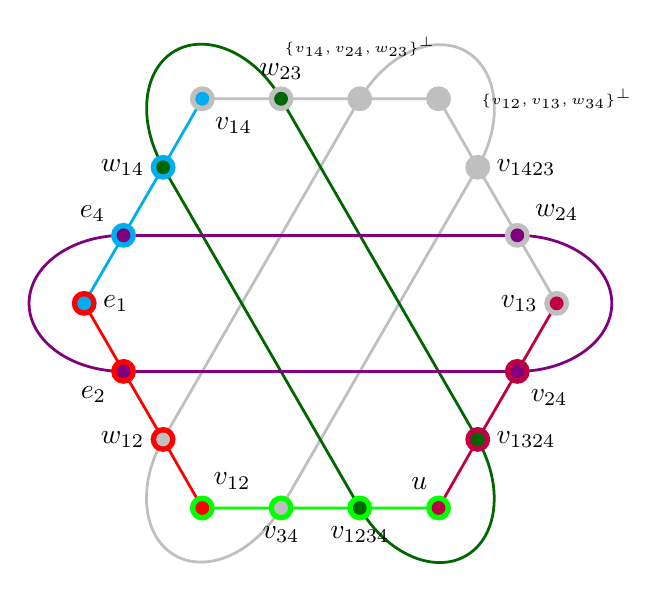
\begin{tikzpicture}  [ultra thick, scale=0.6]

    % --- 1. Define all colors ---
    \colorlet{colorE1E2}{red} \colorlet{colorE4E1}{cyan}
    \colorlet{colorV12V34}{green} \colorlet{colorV13V24}{purple}
    \colorlet{colorCurve24}{violet} \colorlet{lightgray}{gray!50!}
    \colorlet{darkgreen}{green!40!black}

    % --- 2. Define TikZ styles ---
    \tikzstyle{every path}=[line width=1pt]
    \tikzstyle{c2}=[circle,inner sep=3pt,minimum size=9pt]
    \tikzstyle{c1}=[circle,inner sep=0pt,minimum size=5pt]

    % --- 3. Define positions ---
    \path
              (240:5) coordinate(1) (-0.833,-4.33) coordinate(2)
              (0.833,-4.33) coordinate(3) (300:5) coordinate(4)
              (3.33,-2.88) coordinate(5) (4.167,-1.44) coordinate(6)
              (0:5) coordinate(7) (4.167,1.44) coordinate(8)
              (3.33,2.88) coordinate(9) (60:5) coordinate(10)
              (0.833,4.33) coordinate(11) (-0.833,4.33) coordinate(12)
              (120:5) coordinate(13) (-3.33,2.88) coordinate(14)
              (-4.167,1.44) coordinate(15) (180:5) coordinate(16)
              (-4.167,-1.44) coordinate(17) (-3.33,-2.88) coordinate(18);

    % --- 4. Draw context curves ---
    \draw [color=lightgray] (7) -- (8) -- (9)-- (10);
    \draw [color=lightgray] (10) -- (11) -- (12) -- (13);
    \draw [color=lightgray] (9) -- (2); \draw [color=lightgray] (11) -- (18);
    \draw [rotate=240,color=lightgray] (9) arc (90:270:2 and 1.44); \draw[rotate=60,color=lightgray] (18) arc (90:270:2 and 1.44);
    \draw [color=darkgreen] (12) -- (5); \draw [color=darkgreen] (14) -- (3);
    \draw[rotate=300,color=darkgreen] (12) arc (90:270:2 and 1.44); \draw[rotate=120,color=darkgreen] (3) arc (90:270:2 and 1.44);
    \draw [color=colorE4E1] (13) -- (14) -- (15) -- (16);
    \draw [color=colorE1E2] (16) -- (17) -- (18) -- (1);
    \draw [color=colorV12V34] (1) -- (2) -- (3) -- (4);
    \draw [color=colorV13V24] (4) -- (5) -- (6) -- (7);
    \draw [color=colorCurve24] (8) -- (15); \draw [color=colorCurve24](17) -- (6);
    \draw [color=colorCurve24] (8) arc (450:270:2 and 1.44); \draw [color=colorCurve24] (15) arc (90:270:2 and 1.44);

    % --- 5. Draw observables with corrected labels ---
    \draw (1) coordinate[c2,fill=colorV12V34]; \draw (1) coordinate[c1,fill=colorE1E2,label=85:$v_{12}$];
    \draw (2) coordinate[c2,fill=colorV12V34]; \draw (2) coordinate[c1,fill=lightgray,label=270:$v_{34}$];
    \draw (3) coordinate[c2,fill=colorV12V34]; \draw (3) coordinate[c1,fill=darkgreen,label=270:$v_{1234}$];
    \draw (4) coordinate[c2,fill=colorV12V34]; \draw (4) coordinate[c1,fill=colorV13V24,label=95:$u$];
    \draw (5) coordinate[c2,fill=colorV13V24]; \draw (5) coordinate[c1,fill=darkgreen,label=0:$v_{1324}$];
    \draw (6) coordinate[c2,fill=colorV13V24]; \draw (6) coordinate[c1,fill=colorCurve24,label=290:$v_{24}$];
    \draw (7) coordinate[c2,fill=lightgray]; \draw (7) coordinate[c1,fill=colorV13V24,label=180:$v_{13}$];
    \draw (8) coordinate[c2,fill=lightgray]; \draw (8) coordinate[c1,fill=colorCurve24,label=30:$w_{24}$];
    \draw (9) coordinate[c2,fill=lightgray]; \draw (9) coordinate[c1,fill=lightgray,label=0:$v_{1423}$];
    % --- MODIFIED: Explicit construction labels ---
    \draw (10) coordinate[c2,fill=lightgray]; \draw (10) coordinate[c1,fill=lightgray,label={[label distance=3mm,align=center, font=\tiny]0:$\{v_{12}, v_{13}, w_{34}\}^\perp$ }];
    \draw (11) coordinate[c2,fill=lightgray]; \draw (11) coordinate[c1,fill=lightgray,label={[label distance=3mm,align=center, font=\tiny]90:$\{v_{14}, v_{24}, w_{23}\}^\perp$ }];
    \draw (12) coordinate[c2,fill=lightgray]; \draw (12) coordinate[c1,fill=darkgreen,label=90:$w_{23}$];
    \draw (13) coordinate[c2,fill=lightgray]; \draw (13) coordinate[c1,fill=colorE4E1,label=285:$v_{14}$];
    \draw (14) coordinate[c2,fill=colorE4E1]; \draw (14) coordinate[c1,fill=darkgreen,label=180:$w_{14}$];
    \draw (15) coordinate[c2,fill=colorE4E1]; \draw (15) coordinate[c1,fill=colorCurve24,label=160:$e_4$];
    \draw (16) coordinate[c2,fill=colorE1E2]; \draw (16) coordinate[c1,fill=colorE4E1,label=0:$e_1$];
    \draw (17) coordinate[c2,fill=colorE1E2]; \draw (17) coordinate[c1,fill=colorCurve24,label=215:$e_2$];
    \draw (18) coordinate[c2,fill=colorE1E2]; \draw (18) coordinate[c1,fill=lightgray,label=180:$w_{12}$];

\end{tikzpicture}
%}
\\
(a)&&(b)
% \\
% \begin{tikzpicture}[ultra thick, scale=0.35]

%     % --- 1. Define all colors ---
%     \colorlet{colorCircle}{gray}
%     \colorlet{colorE1E2}{red} \colorlet{colorE2E3}{orange}
%     \colorlet{colorE3E4}{blue} \colorlet{colorE4E1}{cyan}
%     \colorlet{colorV12V34}{green} \colorlet{colorV23V41}{lime!70!black}
%     \colorlet{colorCurve13}{magenta} \colorlet{colorCurve24}{violet}
%     \colorlet{colorV13V24}{purple}
%     \colorlet{colorHiddenA}{brown} \colorlet{colorHiddenB}{teal}
%     \colorlet{colorEllipse}{black}   %yellow!80!
%     \colorlet{darkgreen}{green!40!black}

%     % --- 2. Define geometric parameters ---
%     \def\R{10} \def\bendangle{30}

%     % --- 3. Define ALL coordinates first, without drawing ---
% %    \coordinate (u) at (\R/5,0);
%     \foreach \angle/\i in {45/1, 315/2, 225/3, 135/4} { \coordinate (e\i) at (\angle:\R); }
%     \foreach \i/\j in {1/2, 2/3, 3/4, 4/1} {
%         \coordinate (v\i\j) at ($(e\i)!1/3!(e\j)$);
%         \coordinate (w\i\j) at ($(e\i)!2/3!(e\j)$);
%     }
%     \coordinate (v13) at ($(e1)!1/4!(e3)$);
%     \coordinate (v24) at ($(e2)!1/4!(e4)$);
%     \coordinate (w13) at ($(e1)!3/4!(e3)$);
%     \coordinate (w24) at ($(e2)!3/4!(e4)$);
%     \def\vlineangle{63.43}
%     \path[name path=alignment-line] (\vlineangle:\R) -- (\vlineangle+180:\R);
% %    \path[name path=curve-e1-e3] (e1) to[bend right=\bendangle] (e3);
% %    \path[name path=curve-e2-e4] (v23) to[bend right] (v41);
%     \path[name path=curve-v12-v34] (v34) to[bend right] (v12);
%     \path[name path=curve-v23-v14] (v23) to[bend right] (v41);
%     \path[name intersections={of=curve-v12-v34 and curve-v23-v14, by=u}];
% %    \path[name intersections={of=alignment-line and curve-e1-e3, by=v13}];
% %    \path[name intersections={of=alignment-line and curve-e2-e4, by=v24}];
%     \coordinate (g12) at ($(u)!0.5!(v12)$);
%     \coordinate (g13) at ($(u)!0.5!(v13)$);
%     \coordinate (g23) at ($(u)!0.5!(v23)$);
%     \path (e1) (v13)%to[bend right=\bendangle] coordinate[pos=0.85]
%     (w13) (e3);
%     \path (e2) (v24)%to[bend left=\bendangle] coordinate[pos=0.75]
%     (w24) (e4);

%     % --- 4. Draw all lines and curves ---
%     \draw[colorCircle] (0,0) circle (\R);
%     \draw[colorE1E2] (e1) -- (e2); \draw[colorE2E3] (e2) -- (e3);
%     \draw[colorE3E4] (e3) -- (e4); \draw[colorE4E1] (e4) -- (e1);
% %    \draw[colorV12V34] (v12) -- (v34); \draw[colorV23V41] (v23) -- (v41);
%     \draw[colorCurve13] (e1) -- %to[bend right=\bendangle]
%     (e3);
%     \draw[colorCurve24] (e2) -- %to[bend left=\bendangle]
%     (e4);
%     \draw[colorV13V24] (v13) -- (v24);
%     \draw[colorHiddenA] (v41) -- (w23); \draw[colorHiddenA] (w41) -- (v23);
%     \draw[colorHiddenB] (v12) -- (w34); \draw[colorHiddenB] (w12) -- (v34);
%     \draw[colorEllipse] (0,0) circle (\R/2);
% %    \draw[colorEllipse] plot[smooth cycle, tension=0.8] coordinates {(v13) (w24) (w13) (v24)};
%     \draw[colorHiddenA] let \p1=($(w41)-(v41)$), \n1={atan2(\y1,\x1)}, \n2={veclen(\x1,\y1)/2} in (w41) arc (\n1:\n1+180:\n2);
%     \draw[colorHiddenA] let \p1=($(w23)-(v23)$), \n1={atan2(\y1,\x1)}, \n2={veclen(\x1,\y1)/2} in (w23) arc (\n1:\n1+180:\n2);
%     \draw[colorHiddenB] let \p1=($(w12)-(v12)$), \n1={atan2(\y1,\x1)}, \n2={veclen(\x1,\y1)/2} in (w12) arc (\n1:\n1+180:\n2);
%     \draw[colorHiddenB] let \p1=($(w34)-(v34)$), \n1={atan2(\y1,\x1)}, \n2={veclen(\x1,\y1)/2} in (w34) arc (\n1:\n1+180:\n2);

%     \draw[colorV12V34] (v34) to[bend right=\bendangle/3] (v12);
%     \draw[colorV12V34] (v23) to[bend right] (v41);

%     % --- MODIFIED: Emergent block shown with a DOTTED dark green curve ---
%     \draw[darkgreen, dotted, line width=1.5pt] plot[smooth cycle, tension=0.8] coordinates {(w41) %(g13)
%     (w23) (g12)
%     };

%     % --- 5. Draw all points on TOP ---
%     \node[circle, fill=darkgreen, inner sep=2.5pt] at (g13) {};
%     \node[circle, fill=colorV13V24, inner sep=1.5pt, label={left:$v_{1324}$}] at (g13) {};
%     \node[circle, fill=darkgreen, inner sep=2.5pt] at (g12) {};
%     \node[circle, fill=colorV12V34, inner sep=1.5pt, label={below:$v_{1234}$}] at (g12) {};
%     \node[circle, fill=colorV23V41, inner sep=1.5pt, label={above left:$v_{1423}$}] at (g23) {};
%     \node[circle, fill=colorV12V34, inner sep=3pt, label={above left:$u$}] at (u) {}; \node[circle, fill=colorV23V41, inner sep=2pt] at (u) {}; \node[circle, fill=colorV13V24, inner sep=1pt] at (u) {};
% %    \node[circle, fill=colorV12V34, inner sep=3pt, label={above left:$u$}] at (u) {}; \node[circle, fill=colorV23V41, inner sep=2pt] at (u) {}; \node[circle, fill=colorV13V24, inner sep=1pt] at (u) {};
%     \node[circle, fill=colorCurve13, inner sep=3pt, label={above:$v_{13}$}] at (v13) {}; \node[circle, fill=colorV13V24, inner sep=2pt] at (v13) {}; \node[circle, fill=colorEllipse, inner sep=1pt] at (v13) {};
%     \node[circle, fill=colorCurve24, inner sep=3pt, label={below:$v_{24}$}] at (v24) {}; \node[circle, fill=colorV13V24, inner sep=2pt] at (v24) {}; \node[circle, fill=colorEllipse, inner sep=1pt] at (v24) {};
%     \node[circle, fill=colorCurve13, inner sep=2.5pt, label={right:$w_{13}$}] at (w13) {}; \node[circle, fill=colorEllipse, inner sep=1.25pt] at (w13) {};
%     \node[circle, fill=colorCurve24, inner sep=2.5pt, label={below left:$w_{24}$}] at (w24) {}; \node[circle, fill=colorEllipse, inner sep=1.25pt] at (w24) {};
%     \node[circle, fill=darkgreen, inner sep=3.5pt] at (w41) {};
%     \node[circle, fill=colorE4E1, inner sep=2.5pt, label={above right:$w_{14}$}] at (w41) {}; \node[circle, fill=colorHiddenA, inner sep=1.25pt] at (w41) {};
%     \node[circle, fill=darkgreen, inner sep=3.5pt] at (w23) {};
%     \node[circle, fill=colorE2E3, inner sep=2.5pt, label={below left:$w_{23}$}] at (w23) {}; \node[circle, fill=colorHiddenA, inner sep=1.25pt] at (w23) {};
%     \node[circle, fill=colorE4E1, inner sep=3pt, label={above left:$v_{14}$}] at (v41) {}; \node[circle, fill=colorV23V41, inner sep=2pt] at (v41) {}; \node[circle, fill=colorHiddenA, inner sep=1pt] at (v41) {};
%     \node[circle, fill=colorE2E3, inner sep=3pt, label={below right:$v_{23}$}] at (v23) {}; \node[circle, fill=colorV23V41, inner sep=2pt] at (v23) {}; \node[circle, fill=colorHiddenA, inner sep=1pt] at (v23) {};
%     \node[circle, fill=colorE1E2, inner sep=3pt, label={above right:$v_{12}$}] at (v12) {}; \node[circle, fill=colorV12V34, inner sep=2pt] at (v12) {}; \node[circle, fill=colorHiddenB, inner sep=1pt] at (v12) {};
%     \node[circle, fill=colorE1E2, inner sep=2.5pt, label={below right:$w_{12}$}] at (w12) {}; \node[circle, fill=colorHiddenB, inner sep=1.25pt] at (w12) {};
%     \node[circle, fill=colorE3E4, inner sep=3pt, label={below left:$v_{34}$}] at (v34) {}; \node[circle, fill=colorV12V34, inner sep=2pt] at (v34) {}; \node[circle, fill=colorHiddenB, inner sep=1pt] at (v34) {};
%     \node[circle, fill=colorE3E4, inner sep=2.5pt, label={above left:$w_{34}$}] at (w34) {}; \node[circle, fill=colorHiddenB, inner sep=1.25pt] at (w34) {};
%     \node[circle, fill=colorCircle, inner sep=4pt, label={45:$e_1$}] at (e1) {}; \node[circle, fill=colorE4E1, inner sep=3pt] at (e1) {}; \node[circle, fill=colorE1E2, inner sep=2pt] at (e1) {}; \node[circle, fill=colorCurve13, inner sep=1pt] at (e1) {};
%     \node[circle, fill=colorCircle, inner sep=4pt, label={315:$e_2$}] at (e2) {}; \node[circle, fill=colorE1E2, inner sep=3pt] at (e2) {}; \node[circle, fill=colorE2E3, inner sep=2pt] at (e2) {}; \node[circle, fill=colorCurve24, inner sep=1pt] at (e2) {};
%     \node[circle, fill=colorCircle, inner sep=4pt, label={225:$e_3$}] at (e3) {}; \node[circle, fill=colorE2E3, inner sep=3pt] at (e3) {}; \node[circle, fill=colorE3E4, inner sep=2pt] at (e3) {}; \node[circle, fill=colorCurve13, inner sep=1pt] at (e3) {};
%     \node[circle, fill=colorCircle, inner sep=4pt, label={135:$e_4$}] at (e4) {}; \node[circle, fill=colorE3E4, inner sep=3pt] at (e4) {}; \node[circle, fill=colorE4E1, inner sep=2pt] at (e4) {}; \node[circle, fill=colorCurve24, inner sep=1pt] at (e4) {};

% \end{tikzpicture}
% &&
% %\resizebox{0.4\textwidth}{!}{
% \begin{tikzpicture}[thick, scale=0.35]

%     % --- 1. Define all colors ---
%     \colorlet{colorCircle}{gray}
%     \colorlet{colorE1E2}{red} \colorlet{colorE2E3}{orange}
%     \colorlet{colorE3E4}{blue} \colorlet{colorE4E1}{cyan}
%     \colorlet{colorV12V34}{green} \colorlet{colorV23V41}{lime!70!black}
%     \colorlet{colorCurve13}{magenta} \colorlet{colorCurve24}{violet}
%     \colorlet{colorV13V24}{purple}
%     \colorlet{colorHiddenA}{brown} \colorlet{colorHiddenB}{teal}
%     \colorlet{colorEllipse}{black}   %yellow!80!
%     \colorlet{darkgreen}{green!40!black}

%     % --- 2. Define geometric parameters ---
%     \def\R{10} \def\bendangle{30}

%     % --- 3. Define ALL coordinates first, without drawing ---
%     \coordinate (u) at (0,0);
%     \foreach \angle/\i in {45/1, 315/2, 225/3, 135/4} { \coordinate (e\i) at (\angle:\R); }
%     \foreach \i/\j in {1/2, 2/3, 3/4, 4/1} {
%         \coordinate (v\i\j) at ($(e\i)!1/3!(e\j)$);
%         \coordinate (w\i\j) at ($(e\i)!2/3!(e\j)$);
%     }
%     \def\vlineangle{63.43}
%     \path[name path=alignment-line] (\vlineangle:\R) -- (\vlineangle+180:\R);
%     \path[name path=curve-e1-e3] (e1) to[bend right=\bendangle] (e3);
%     \path[name path=curve-e2-e4] (e2) to[bend left=\bendangle] (e4);
%     \path[name intersections={of=alignment-line and curve-e1-e3, by=v13}];
%     \path[name intersections={of=alignment-line and curve-e2-e4, by=v24}];
%     \coordinate (g13) at ($(u)!0.5!(v13)$); \coordinate (g12) at ($(u)!0.5!(v12)$);
%     \coordinate (g23) at ($(u)!0.5!(v23)$);
%     \path (e1) to[bend right=\bendangle] coordinate[pos=0.85] (w13) (e3);
%     \path (e2) to[bend left=\bendangle] coordinate[pos=0.75] (w24) (e4);

%     % --- 4. Draw all lines and curves ---
%     \draw[colorCircle] (0,0) circle (\R);
%     \draw[colorE1E2] (e1) -- (e2); \draw[colorE2E3] (e2) -- (e3);
%     \draw[colorE3E4] (e3) -- (e4); \draw[colorE4E1] (e4) -- (e1);
%     \draw[colorV12V34] (v12) -- (v34); \draw[colorV23V41] (v23) -- (v41);
%     \draw[colorCurve13] (e1) to[bend right=\bendangle] (e3);
%     \draw[colorCurve24] (e2) to[bend left=\bendangle] (e4);
%     \draw[colorV13V24] (v13) -- (v24);
%     \draw[colorHiddenA] (v41) -- (w23); \draw[colorHiddenA] (w41) -- (v23);
%     \draw[colorHiddenB] (v12) -- (w34); \draw[colorHiddenB] (w12) -- (v34);
%     \draw[colorEllipse] plot[smooth cycle, tension=0.8] coordinates {(v13) (w24) (w13) (v24)};
%     \draw[colorHiddenA] let \p1=($(w41)-(v41)$), \n1={atan2(\y1,\x1)}, \n2={veclen(\x1,\y1)/2} in (w41) arc (\n1:\n1+180:\n2);
%     \draw[colorHiddenA] let \p1=($(w23)-(v23)$), \n1={atan2(\y1,\x1)}, \n2={veclen(\x1,\y1)/2} in (w23) arc (\n1:\n1+180:\n2);
%     \draw[colorHiddenB] let \p1=($(w12)-(v12)$), \n1={atan2(\y1,\x1)}, \n2={veclen(\x1,\y1)/2} in (w12) arc (\n1:\n1+180:\n2);
%     \draw[colorHiddenB] let \p1=($(w34)-(v34)$), \n1={atan2(\y1,\x1)}, \n2={veclen(\x1,\y1)/2} in (w34) arc (\n1:\n1+180:\n2);

%     % --- MODIFIED: Emergent block shown with a DOTTED dark green curve ---
%     \draw[darkgreen, dotted, line width=1.5pt] plot[smooth cycle, tension=0.8] coordinates {(w41) (g13) (w23) (g12)};

%     % --- 5. Draw all points on TOP ---
%     \node[circle, fill=darkgreen, inner sep=2.5pt] at (g13) {};
%     \node[circle, fill=colorV13V24, inner sep=1.5pt, label={left:$v_{1324}$}] at (g13) {};
%     \node[circle, fill=darkgreen, inner sep=2.5pt] at (g12) {};
%     \node[circle, fill=colorV12V34, inner sep=1.5pt, label={below:$v_{1234}$}] at (g12) {};
%     \node[circle, fill=colorV23V41, inner sep=1.5pt, label={above left:$v_{1423}$}] at (g23) {};
%     \node[circle, fill=colorV12V34, inner sep=3pt, label={above left:$u$}] at (u) {}; \node[circle, fill=colorV23V41, inner sep=2pt] at (u) {}; \node[circle, fill=colorV13V24, inner sep=1pt] at (u) {};
%     \node[circle, fill=colorCurve13, inner sep=3pt, label={above:$v_{13}$}] at (v13) {}; \node[circle, fill=colorV13V24, inner sep=2pt] at (v13) {}; \node[circle, fill=colorEllipse, inner sep=1pt] at (v13) {};
%     \node[circle, fill=colorCurve24, inner sep=3pt, label={below:$v_{24}$}] at (v24) {}; \node[circle, fill=colorV13V24, inner sep=2pt] at (v24) {}; \node[circle, fill=colorEllipse, inner sep=1pt] at (v24) {};
%     \node[circle, fill=colorCurve13, inner sep=2.5pt, label={right:$w_{13}$}] at (w13) {}; \node[circle, fill=colorEllipse, inner sep=1.25pt] at (w13) {};
%     \node[circle, fill=colorCurve24, inner sep=2.5pt, label={below left:$w_{24}$}] at (w24) {}; \node[circle, fill=colorEllipse, inner sep=1.25pt] at (w24) {};
%     \node[circle, fill=darkgreen, inner sep=3.5pt] at (w41) {};
%     \node[circle, fill=colorE4E1, inner sep=2.5pt, label={above right:$w_{14}$}] at (w41) {}; \node[circle, fill=colorHiddenA, inner sep=1.25pt] at (w41) {};
%     \node[circle, fill=darkgreen, inner sep=3.5pt] at (w23) {};
%     \node[circle, fill=colorE2E3, inner sep=2.5pt, label={below left:$w_{23}$}] at (w23) {}; \node[circle, fill=colorHiddenA, inner sep=1.25pt] at (w23) {};
%     \node[circle, fill=colorE4E1, inner sep=3pt, label={above left:$v_{14}$}] at (v41) {}; \node[circle, fill=colorV23V41, inner sep=2pt] at (v41) {}; \node[circle, fill=colorHiddenA, inner sep=1pt] at (v41) {};
%     \node[circle, fill=colorE2E3, inner sep=3pt, label={below right:$v_{23}$}] at (v23) {}; \node[circle, fill=colorV23V41, inner sep=2pt] at (v23) {}; \node[circle, fill=colorHiddenA, inner sep=1pt] at (v23) {};
%     \node[circle, fill=colorE1E2, inner sep=3pt, label={above right:$v_{12}$}] at (v12) {}; \node[circle, fill=colorV12V34, inner sep=2pt] at (v12) {}; \node[circle, fill=colorHiddenB, inner sep=1pt] at (v12) {};
%     \node[circle, fill=colorE1E2, inner sep=2.5pt, label={below right:$w_{12}$}] at (w12) {}; \node[circle, fill=colorHiddenB, inner sep=1.25pt] at (w12) {};
%     \node[circle, fill=colorE3E4, inner sep=3pt, label={below left:$v_{34}$}] at (v34) {}; \node[circle, fill=colorV12V34, inner sep=2pt] at (v34) {}; \node[circle, fill=colorHiddenB, inner sep=1pt] at (v34) {};
%     \node[circle, fill=colorE3E4, inner sep=2.5pt, label={above left:$w_{34}$}] at (w34) {}; \node[circle, fill=colorHiddenB, inner sep=1.25pt] at (w34) {};
%     \node[circle, fill=colorCircle, inner sep=4pt, label={45:$e_1$}] at (e1) {}; \node[circle, fill=colorE4E1, inner sep=3pt] at (e1) {}; \node[circle, fill=colorE1E2, inner sep=2pt] at (e1) {}; \node[circle, fill=colorCurve13, inner sep=1pt] at (e1) {};
%     \node[circle, fill=colorCircle, inner sep=4pt, label={315:$e_2$}] at (e2) {}; \node[circle, fill=colorE1E2, inner sep=3pt] at (e2) {}; \node[circle, fill=colorE2E3, inner sep=2pt] at (e2) {}; \node[circle, fill=colorCurve24, inner sep=1pt] at (e2) {};
%     \node[circle, fill=colorCircle, inner sep=4pt, label={225:$e_3$}] at (e3) {}; \node[circle, fill=colorE2E3, inner sep=3pt] at (e3) {}; \node[circle, fill=colorE3E4, inner sep=2pt] at (e3) {}; \node[circle, fill=colorCurve13, inner sep=1pt] at (e3) {};
%     \node[circle, fill=colorCircle, inner sep=4pt, label={135:$e_4$}] at (e4) {}; \node[circle, fill=colorE3E4, inner sep=3pt] at (e4) {}; \node[circle, fill=colorE4E1, inner sep=2pt] at (e4) {}; \node[circle, fill=colorCurve24, inner sep=1pt] at (e4) {};

% \end{tikzpicture}
% %}
\end{tabular}
\caption{
\rev{(a) Four-dimensional extension of the Harding--Salinas Schmeis hypergraph notation~\cite{harding2025remarksIJTP}.  Solid curves show imposed contexts.  The dotted dark-green curve is the equality-induced context $\mathcal{E}_3=\{w_{14},w_{23},v_{1234},v_{1324}\}$; the other contexts of the complete $20$-ray orthogonality hypergraph are listed in the text.  (b) The Cabello $18$-ray, $9$-context KS configuration~\cite{cabello-96}, with labels from Ref.~\cite{cabello:210401}.  Shared rays are relabeled by the gadget notation; overall nonzero scalar factors are immaterial.  The notation $\{v_i,v_j,v_k\}^{\perp}$ denotes the unique ray orthogonal to the span of three independent rays.  The drawings record the stated incidence relations; no lattice-theoretic conclusion is inferred from the planar layout alone.}
}
\label{fig:peres}
\end{figure*}




\begin{table*}[ht]
\caption{\rev{Comparison of the $20$-ray gadget and the Cabello $18$-ray set~\cite{cabello-96,cabello:210401}.  Both lie in the $24$-ray Peres--Mermin eigensystem~\cite{peres111,mermin90b,peres-91,pavicic-2004ksafq,svozil-2024-convert-pra-externalfigures}.  Fifteen rays are shared projectively.  Each of the five gadget-only rays and each of the three Cabello-only rays is the unique orthogonal complement of a three-dimensional span generated by the other set, establishing mutual reconstructibility.}}
\label{tab:vector-equivalence}
\begin{ruledtabular}
\begin{tabular}{cccc}
Gadget Label & Gadget Vector & Cabello Diagram Label & Vector Construction / Definition \\
\hline
$u$ & $(1,1,1,1)$ & $v_{56}$ & $(1,1,1,1)$ \\
$e_1$ & $(1,0,0,0)$ & $v_{12}$ & $(1,0,0,0)$ \\
$e_2$ & $(0,1,0,0)$ & $v_{18}$ & $(0,1,0,0)$ \\
$e_3$ & $(0,0,1,0)$ & (Constructed) & $\{v_{12}, v_{18}, v_{28}\}^\perp$ \\
$e_4$ & $(0,0,0,1)$ & $v_{28}$ & $(0,0,0,1)$ \\
\hline
$v_{12}$ & $(0,0,1,-1)$ & $v_{16}$ & $(0,0,1,-1)$ \\
$v_{13}$ & $(0,-1,0,1)$ & $v_{45}$ & $(0,1,0,-1)$ \\
$v_{14}$ & $(0,1,-1,0)$ & $v_{23}$ & $(0,1,-1,0)$ \\
$v_{23}$ & $(1,0,0,-1)$ & \rev{(Constructed)} & \rev{$\{v_{18},v_{23},v_{39}\}^\perp$} \\
$v_{24}$ & $(-1,0,1,0)$ & $v_{58}$ & $(1,0,-1,0)$ \\
$v_{34}$ & $(1,-1,0,0)$ & $v_{67}$ & $(1,-1,0,0)$ \\
\hline
$w_{12}$ & $(0,0,1,1)$ & $v_{17}$ & $(0,0,1,1)$ \\
$w_{13}$ & $(0,1,0,1)$ & \rev{(Constructed)} & \rev{$\{v_{12},v_{45},v_{58}\}^\perp$} \\
$w_{14}$ & $(0,1,1,0)$ & $v_{29}$ & $(0,1,1,0)$ \\
$w_{23}$ & $(1,0,0,1)$ & $v_{39}$ & $(1,0,0,1)$ \\
$w_{24}$ & $(1,0,1,0)$ & $v_{48}$ & $(1,0,1,0)$ \\
$w_{34}$ & $(1,1,0,0)$ & \rev{(Constructed)} & \rev{$\{v_{28},v_{16},v_{67}\}^\perp$} \\
\hline
$v_{1234}$ & $(1,1,-1,-1)$ & $v_{69}$ & $(1,1,-1,-1)$ \\
$v_{1324}$ & $(1,-1,1,-1)$ & $v_{59}$ & $(1,-1,1,-1)$ \\
$v_{1423}$ & $(1,-1,-1,1)$ & \rev{(Constructed)} & \rev{$\{v_{23},v_{17},v_{48}\}^\perp$} \\
\hline
(Constructed) & $\{v_{12}, v_{13}, w_{34}\}^\perp$ & $v_{34}$ & $(-1,1,1,1)$ \\
(Constructed) & $\{v_{14}, v_{24}, w_{23}\}^\perp$ & $v_{37}$ & $(1,1,1,-1)$ \\
\rev{(Constructed)} & \rev{$\{v_{13},v_{23},w_{12}\}^\perp$} & \rev{$v_{47}$} & \rev{$(1,1,-1,1)$} \\
\end{tabular}
\end{ruledtabular}
\end{table*}





\subsubsection{Concrete $D=4$ example: $u=(1,1,1,1)$}

Take the center vector $u=(1,1,1,1)$ and the rim vectors
\begin{align*}
e_1&=(1,0,0,0),& e_2 =(0,1,0,0),\\
e_3&=(0,0,1,0),& e_4 =(0,0,0,1).
\end{align*}
The pair minors and their complementary vectors become:
\begin{align*}
v_{12}&=(0,0,1,-1), & w_{12}&=(0,0,1,1),\\
v_{13}&=(0,-1,0,1), & w_{13}&=(0,1,0,1),\\
v_{14}&=(0,1,-1,0), & w_{14}&=(0,1,1,0),\\
v_{23}&=(1,0,0,-1), & w_{23}&=(1,0,0,1),\\
v_{24}&=(-1,0,1,0), & w_{24}&=(1,0,1,0),\\
v_{34}&=(1,-1,0,0), & w_{34}&=(1,1,0,0).
\end{align*}
Each pair block
\[
\mathcal{B}_{ij}=\{e_i, e_j, v_{ij}, w_{ij}\}
\]
forms an ONB after normalizing $v_{ij}$ and $w_{ij}$.

The connector vectors are
\begin{align*}
v_{1234}&=(1,1,-1,-1),\\
v_{1324}& =(1,-1,1,-1),\\
v_{1423}&=(1,-1,-1,1),
\end{align*}
and they are all orthogonal to $u=(1,1,1,1)$ by inspection.

A convenient explicit completion of the connector blocks can be formed using some of the existing minor vectors:
\begin{align*}
C_{(a)}&=\{u, v_{1234}, v_{34}, v_{12}\},\\
C_{(b)}&=\{u, v_{1324}, v_{24}, v_{13}\},\\
C_{(c)}&=\{u, v_{1423}, v_{23}, v_{14}\}.
\end{align*}
Each of these sets is composed of four mutually orthogonal vectors. For example, in $C_{(a)}$, the vectors $v_{34}$ and $v_{12}$ have disjoint support,
making them orthogonal. The inner products $\langle v_{1234}, v_{34} \rangle$ and $\langle v_{1234}, v_{12} \rangle$ are zero, as are all other inner products involving $u$. To create literal ONBs, the vectors should be normalized.

\rev{Together with $\mathcal{B}_{\mathrm{comp}}$, the six pair contexts and three connector contexts form the 10-context scaffold that enforces Proposition~\ref{prop:D4forcing}.  The equal-modulus condition also creates $\mathcal{C}_0$ and the three contexts $\mathcal{E}_1,\mathcal{E}_2,\mathcal{E}_3$ listed above.  For example, $\langle w_{14},v_{1234}\rangle=|x_2|^2-|x_3|^2=0$; $\mathcal{E}_3$ is the dotted dark-green curve in Fig.~\ref{fig:peres}(a).}


\begin{revision}
\subsubsection{Mutual reconstruction inside the Peres--Mermin eigensystem}

Both ray sets are subsets of the $24$-ray Peres--Mermin eigensystem~\cite{pavicic-2004ksafq,svozil-2024-convert-pra-externalfigures}.  They share $15$ rays projectively.  Table~\ref{tab:vector-equivalence} gives rank-three orthogonal-complement constructions for the five gadget-only rays and the three Cabello-only rays.  Hence each ray set generates the other under the operation ``take the unique ray orthogonal to three independent rays.''  This is the precise sense in which we call them informationally equivalent.

Informational equivalence does not imply equality of context hypergraphs.  The complete $20$-ray orthogonality hypergraph has $17$ contexts and $16$ separating two-valued states.  The Cabello $18$-ray hypergraph selects nine contexts and has no two-valued state; its parity argument makes it a KS configuration~\cite{cabello-96}.  The contrast is therefore not a consequence of ``more contexts allowing loopholes''---adding constraints cannot create two-valued states---but of the two constructions selecting different rays and different contexts from their common $24$-ray parent.

\subsubsection{Context completion and two-valued states}

The context choice within the $20$-ray set can itself be tracked explicitly.  Let
\[
\mathfrak{B}_{10}=\{\mathcal{B}_{\mathrm{comp}},\mathcal{B}_{ij}\ (1\leq i<j\leq4),
\mathcal{C}_{(a)},\mathcal{C}_{(b)},\mathcal{C}_{(c)}\}
\]
be the 10 imposed contexts, and let
\[
\mathfrak{B}_{13}=\mathfrak{B}_{10}\cup
\{\mathcal{B}_{1234},\mathcal{B}_{1324},\mathcal{B}_{1423}\}.
\]
Exact enumeration shows that both hypergraphs have the same $36$ two-valued states, and those states are separating.  The three disjoint-support contexts therefore record exclusions already obeyed by every state of $\mathfrak{B}_{10}$; they do not remove an assignment.  Adding the four equality-induced contexts gives the complete set
\[
\mathfrak{B}_{17}=\mathfrak{B}_{13}\cup\{\mathcal{C}_0,\mathcal{E}_1,\mathcal{E}_2,\mathcal{E}_3\},
\]
which has $16$ separating two-valued states.  This nested comparison makes the monotonicity transparent: adding contexts can preserve or reduce the state set, but cannot enlarge it.  It also avoids attributing KS contextuality to an incomplete incidence structure merely because some available contexts were omitted.

The apparent asymmetry of Fig.~\ref{fig:peres}(a) is mainly graphical and reflects the selected $20$-ray subset.  Both it and the Cabello $18$-ray set sit inside the more symmetric $24$-ray, $24$-context Peres configuration~\cite{Pavicic-2005,pavicic-2005csvcorri}; neither subset needs to
inherit all symmetries of the parent.
\end{revision}


\begin{revision}
\subsection{A $D=5$ scaffold and forcing constraint}

Let $\varepsilon_{abcde}$ be a totally antisymmetric tensor
with $\varepsilon_{12345}=1$.  For each triple $\{i,j,k\}$ define
\[
(v_{ijk})_m=\sum_{\ell=1}^5\varepsilon_{mijk\ell}\,\overline{x_\ell}.
\]
The vector $v_{ijk}$ vanishes in coordinates $i,j,k$ and satisfies $\langle v_{ijk},u\rangle=0$ by antisymmetry.  Choose $w_{ijk}$ on the complementary two coordinates with $v_{ijk}\perp w_{ijk}$; then
\[
\mathcal{B}_{ijk}=\{e_i,e_j,e_k,v_{ijk},w_{ijk}\}
\]
is a scaffold context.

The four connector rays are represented by
\begin{align*}
g_1&=(x_1,0,0,0,-x_5),&
g_2&=(0,x_2,0,0,-x_5),\\
g_3&=(0,0,x_3,0,-x_5),&
g_4&=(0,0,0,x_4,-x_5).
\end{align*}
Whenever $u\perp g_i$, three rays spanning $\operatorname{span}\{u,g_i\}^{\perp}$ complete the connector context $\mathcal{C}_i=\{u,g_i,h^{(i)}_1,h^{(i)}_2,h^{(i)}_3\}$.

\begin{proposition}[$D=5$ forcing constraint]
\label{prop:D5forcing}
The four connector contexts force a normalized center vector $u$ to be maximally unbiased relative to the computational basis.
\end{proposition}

\begin{proof}
For $i=1,2,3,4$,
\[
\langle u,g_i\rangle=|x_i|^2-|x_5|^2.
\]
Thus the four orthogonality conditions imply \ensuremath{|x_1|=\cdots=|x_5|};
normalization makes every squared modulus $1/5$.
\end{proof}
\end{revision}

\section{Summary and Conclusion}

%\subsection{Summary}

\begin{revision}
The qutrit construction yields $165$ projectively distinct rays and exactly $130$ contexts.  Correct provenance accounting is symmetric: the three $69$-ray, $50$-context KS lineages share $21$ rays and $10$ contexts, and each adds $48$ exclusive rays and $40$ lineage-specific contexts.  This places the triple of $25$-ray full-context Yu--Oh completions, Harding--Salinas Schmeis, and Cabello descriptions in a common MUB-based framework without assigning shared rays to an arbitrary first lineage.

In $D=4$ and $D=5$, the forcing mechanism is explicit at the level of constraints: connector orthogonalities yield linear equations in the squared coordinate moduli and hence maximal unbiasedness.  For the concrete $D=4$ realization, the complete $20$-ray orthogonality hypergraph has $17$ contexts and $16$ separating two-valued states.  Its ray set is mutually reconstructible with the Cabello $18$-ray set inside the $24$-ray Peres--Mermin eigensystem, but the Cabello nine-context hypergraph is uncolorable.  Ray-set closure and context incidence are therefore distinct pieces of data.

The main methodological conclusion is that contextuality claims should specify the incidence hypergraph being tested and, when completeness is intended, enumerate every context supported by the chosen rays.  Restricting attention to intertwining rays or to a selected subset of available contexts may define a legitimate reduced scenario, but its two-valued-state properties should not be transferred to a different completion without a separate check.
\end{revision}

\begin{acknowledgments}
We are grateful to Josef Tkadlec for providing a {\em Pascal} program that computes and analyses the set of two-valued states of collections of contexts.
We are also grateful to Ad\'{a}n Cabello and Mladen Pavi{\v{c}}i{\'{c}} for valuable communications.

\rev{OpenAI Codex (GPT-5) was used to assist with literature organization, \LaTeX{}
editing, and checks of derivations.  The authors
specified the scientific
direction and prompts; model output retained in the manuscript was checked
against the cited sources and explicit calculations.  The authors accept
full
responsibility for the final text.}

This research was funded in part by the Austrian
Science Fund (FWF), Grant DOI \href{https://doi.org/10.55776/PIN5424624}{10.55776/PIN5424624},
and the Czech Science
Foundation (GA\v{C}R), Grant No.~25-20013L.

The authors declare no conflict of interest.
\end{acknowledgments}

\bibliography{svozil}

\bigskip
\appendix

\begin{revision}
\section{Mutually unbiased bases in $\mathbb{C}^3$}
\label{appendix:MUBsD3}

For introductions to MUBs, see Refs.~\cite{Schwinger.60,WooFie,Brierley2009,springerlink:10.1007/978-3-540-24633-6_10,durt,mcnulty2024mutually}.  Write
\[
\omega=\mathrm{e}^{2\pi\ii{}/3},\qquad
\omega^3=1,\qquad 1+\omega+\omega^2=0,
\qquad \overline{\omega}=\omega^2.
\]
In $D=3$, a complete MUB family contains four bases~\cite{ivanovic-1997}.  Omitting the common normalization factor $1/\sqrt{3}$ from the last three bases, we use
\begin{align}
\mathcal{B}_0&=\{(1,0,0),(0,1,0),(0,0,1)\}, \label{eq:B0_3}\\
\mathcal{B}_1&=\{(1,1,1),(1,\omega,\omega^2),(1,\omega^2,\omega)\}, \label{eq:B1_3}\\
\mathcal{B}_2&=\{(1,\omega,\omega),(1,\omega^2,1),(1,1,\omega^2)\}, \label{eq:B2_3}\\
\mathcal{B}_3&=\{(1,\omega^2,\omega^2),(1,\omega,1),(1,1,\omega)\}. \label{eq:B3_3}
\end{align}
Here $\mathcal{B}_0$ is computational and $\mathcal{B}_1$ is the Fourier basis.  Direct use of $1+\omega+\omega^2=0$ verifies orthogonality within each basis and $|\langle b,b'\rangle|^2=1/3$ between normalized vectors from different bases.  The ordering of $\mathcal{B}_2$ and $\mathcal{B}_3$ agrees with the \ensuremath{\sigma_j} seed groups in Table~\ref{tab:vector_generation}.

For the higher-dimensional argument, no catalogue of a complete MUB family is required: Propositions~\ref{prop:D4forcing} and~\ref{prop:D5forcing} use only the criterion \ensuremath{|x_1|=\cdots=|x_D|} for one vector to be maximally unbiased relative to the computational basis.
\end{revision}





\end{document}

~~~~~~~~~~~~~~~~~~~~~~~~~~~~~~~~~~~~~~~~~~~~~~~~~~~~~~~~~~~~~~~~~~~~~~~~~~~~~~~~~~~~~~~~

(* ::Section:: *)
(* Symmetric MUB analysis with projective collinearity + orthogonal bases + LaTeX export *)
(* Version: Final, with professional label formatting a_2[1] -> $a_{21}$ *)

(* Clean slate *)
ClearAll["Global`*"];

(* ---------- Core symbols and pretty printing ---------- *)
w = Exp[2 Pi I/3];
toOmegaRules = {Exp[(2 Pi I)/3] -> \[Omega], Exp[(-2 Pi I)/3] -> \[Omega]^2, Exp[(4 Pi I)/3] -> \[Omega]^2, Exp[(-4 Pi I)/3] -> \[Omega], Conjugate[Exp[(2 Pi I)/3]] -> \[Omega]^2, Conjugate[Exp[(-2 Pi I)/3]] -> \[Omega], Conjugate[Exp[(4 Pi I)/3]] -> \[Omega], Conjugate[Exp[(-4 Pi I)/3]] -> \[Omega]^2, w -> \[Omega], w^2 -> \[Omega]^2, Conjugate[w] -> \[Omega]^2, Conjugate[w^2] -> \[Omega]};
assum = {w^3 == 1, w != 1, 1 + w + w^2 == 0, Conjugate[w] == w^2, Conjugate[w^2] == w};
pretty[expr_] := Simplify[expr /. toOmegaRules, Assumptions -> assum] /. toOmegaRules;

(* ---------- Utility: projective canonical representative & collinearity ---------- *)
ZeroVectorQ[v_List] := TrueQ[Simplify[v == {0, 0, 0}, Assumptions -> assum]];
CanonicalDir[v_List] := Module[{v2 = Simplify[v, Assumptions -> assum], pos}, If[ZeroVectorQ[v2], {0, 0, 0}, pos = First@First@Position[Map[Simplify[# != 0, Assumptions -> assum] &, v2], True]; Simplify[v2/v2[[pos]], Assumptions -> assum]]];
UniqueCountNonCollinear[vecs_List] := Length@GatherBy[vecs, CanonicalDir];

(* ---------- Index helpers and symmetric family definitions (unchanged) ---------- *)
e[1] = {1, 0, 0}; e[2] = {0, 1, 0}; e[3] = {0, 0, 1};
others2[i_Integer] := Complement[{1, 2, 3}, {i}];
a[i_Integer][_ : Null] := e[i];
uF[{x_, y_, z_}] := {x, y, z};
b[i_Integer][{x_, y_, z_}] := ReplacePart[{x, y, z}, i -> 0];
c[i_Integer][u_List] := -Conjugate[Cross[e[i], u]];
d[i_Integer][u : {x_, y_, z_}] := Module[{j, k, lst = {x, y, z}}, {j, k} = others2[i]; ReplacePart[ConstantArray[0, 3], {i -> -(lst[[j]] Conjugate[lst[[j]]] + lst[[k]] Conjugate[lst[[k]]]), j -> Conjugate[lst[[i]]] lst[[j]], k -> Conjugate[lst[[i]]] lst[[k]]}]];
b12[{x_, y_, z_}] := {Conjugate[y z], Conjugate[x z], -Conjugate[x y]};
b13[{x_, y_, z_}] := {Conjugate[y z], -Conjugate[x z], Conjugate[x y]};
b23[{x_, y_, z_}] := {-Conjugate[y z], Conjugate[x z], Conjugate[x y]};
CCross[u_List, v_List] := Conjugate[Cross[u, v]];
eF[1][uvw_] := CCross[c[2][uvw], b13[uvw]];
eF[2][uvw_] := CCross[c[3][uvw], b12[uvw]];
eF[3][uvw_] := CCross[c[1][uvw], b23[uvw]];
b112[{x_, y_, z_}] := {x y Conjugate[y] + x z Conjugate[z], -y z Conjugate[z], y Conjugate[y] z};
b212[{x_, y_, z_}] := {-x z Conjugate[z], x Conjugate[x] y + y z Conjugate[z], x Conjugate[x] z};
b113[{x_, y_, z_}] := {x y Conjugate[y] + x z Conjugate[z], y z Conjugate[z], -y Conjugate[y] z};
b313[{x_, y_, z_}] := {-x y Conjugate[y], x Conjugate[x] y, x Conjugate[x] z + y Conjugate[y] z};
b223[{x_, y_, z_}] := {x z Conjugate[z], y z Conjugate[z] + x Conjugate[x] y, -x Conjugate[x] z};
b323[{x_, y_, z_}] := {x y Conjugate[y], -x Conjugate[x] y, x Conjugate[x] z + y Conjugate[y] z};
labelsAndFns = {{"a_1", a[1]}, {"a_2", a[2]}, {"a_3", a[3]}, {"u", uF}, {"b_1", b[1]}, {"b_2", b[2]}, {"b_3", b[3]}, {"c_1", c[1]}, {"c_2", c[2]}, {"c_3", c[3]}, {"d_1", d[1]}, {"d_2", d[2]}, {"d_3", d[3]}, {"b_{12}", b12}, {"b_{13}", b13}, {"b_{23}", b23}, {"e_1", eF[1]}, {"e_2", eF[2]}, {"e_3", eF[3]}, {"b_{112}", b112}, {"b_{212}", b212}, {"b_{113}", b113}, {"b_{313}", b313}, {"b_{223}", b223}, {"b_{323}", b323}};
sets = {{1, 1, 1}, {1, w, w^2}, {1, w^2, w}, {1, w, w}, {1, w^2, 1}, {1, 1, w^2}, {1, w^2, w^2}, {1, w, 1}, {1, 1, w}};

(* ========== Label Formatting Helper (*NEW*) ========== *)
formatLabelAsTeX[str_String] := Module[{name, subscript, index},
  If[StringContainsQ[str, "["],
    (* It's a generated vector label like a_2[1] or u[5] *)
    name = StringSplit[str, {"_", "["}][[1]];
    index = StringCases[str, "[" ~~ i__ ~~ "]" :> i][[1]];
    subscript = If[StringContainsQ[str, "_"],
      StringDelete[StringCases[str, "_" ~~ s__ ~~ "[" :> s][[1]], {"{", "}"}],
      ""
    ];
    "$" <> name <> "_{" <> subscript <> index <> "}$"
    ,
    (* It's a base function label like a_1 or b_{12} *)
    "$" <> StringReplace[str, "_" -> "_"] <> "$"
  ]
];

(* ---------- (1) Row-wise table with projective non-collinearity counts ---------- *)
table1Rows = labelsAndFns /. {label_, f_} :> Module[{vecsRaw = f /@ sets, count}, count = UniqueCountNonCollinear[vecsRaw]; Join[{label}, pretty /@ vecsRaw, {count}]];
table1 = Prepend[table1Rows, Join[{"Label"}, Table["u" <> ToString[i], {i, Length[sets]}], {"# Non-collinear"}]];
Print[Style["Table 1: Row-wise Non-collinearity Counts", Bold, 14]];
Grid[table1, Frame -> All, ItemSize -> All, Spacings -> {2, 1}, Background -> {None, {LightGray, None}}]

(* ---------- (2) Global non-collinear set with labels ---------- *)
allLabeled = Flatten[Table[{labelsAndFns[[k, 1]] <> "[" <> ToString[i] <> "]", labelsAndFns[[k, 2]][sets[[i]]]}, {k, Length[labelsAndFns]}, {i, Length[sets]}], 1];
allLabeledWithCanon = Table[{vec[[1]], vec[[2]], CanonicalDir[vec[[2]]]}, {vec, allLabeled}];
globalClasses = GatherBy[allLabeledWithCanon, Last];
uniqueLabeledVectors = {#[[1]], #[[2]]} & /@ (First /@ globalClasses);
(* >> REVISED: Create a display-ready version of the table with new label format *)
displayTable2 = Prepend[({formatLabelAsTeX[#[[1]]], pretty@#[[2]]} & /@ uniqueLabeledVectors), {"Label", "Vector"}];
Print["\n", Style["Table 2: Globally Unique Non-Collinear Vectors", Bold, 14]];
Grid[displayTable2, Frame -> All, ItemSize -> All, Spacings -> {2, 1}, Background -> {None, {LightGray, None}}]
Print[Style["\n(1) Total number of global non-collinear vectors: ", Bold], Length[uniqueLabeledVectors]];

(* ---------- (3) Orthogonal bases among globally unique vectors ---------- *)
OrthogonalQ[v1_, v2_] := TrueQ[Simplify[v1 . Conjugate[v2] == 0, Assumptions -> assum]];
nonZeroUniques = Select[uniqueLabeledVectors, !ZeroVectorQ[#[[2]]]&];
numUniques = Length[nonZeroUniques];
Print["\nBuilding orthogonality graph..."];
orthoLists = Monitor[Table[v1 = nonZeroUniques[[i, 2]]; Select[Range[i + 1, numUniques], OrthogonalQ[v1, nonZeroUniques[[#, 2]]]&], {i, 1, numUniques}], "Processing vector " <> ToString[i] <> "/" <> ToString[numUniques]];
Print["Graph built. Searching for bases..."];
Module[{result}, result = Last@Reap[Monitor[Do[Module[{neighborsOfI}, neighborsOfI = orthoLists[[i]]; If[Length[neighborsOfI] < 2, Continue[]]; Do[Module[{j, neighborsOfJ, commonNeighborsK}, j = neighborsOfI[[jIdx]]; neighborsOfJ = orthoLists[[j]]; commonNeighborsK = Intersection[neighborsOfI, neighborsOfJ]; Do[Sow[{nonZeroUniques[[i]], nonZeroUniques[[j]], nonZeroUniques[[k]]}], {k, commonNeighborsK}]], {jIdx, 1, Length[neighborsOfI]}]], {i, 1, numUniques}], "Searching for bases starting with vector " <> ToString[i] <> "/" <> ToString[numUniques]]]; orthBases = If[result === {}, {}, First[result]];];
(* >> REVISED: Create a display-ready version of the table with new label format *)
displayTable3 = Prepend[({StringRiffle[formatLabelAsTeX /@ #[[All, 1]], ", "]} & /@ orthBases), {"Orthogonal Basis (Labels)"}];
Print["\n", Style["Table 3: Orthogonal Bases Found", Bold, 14]];
Grid[displayTable3, Frame -> All, ItemSize -> All, Spacings -> {2, 1}, Background -> {None, {LightGray, None}}]
Print[Style["\n(2) Total number of orthogonal bases: ", Bold], Length[orthBases]];


(* ========== LaTeX helpers and exports (*REVISED*) ========== *)
Print["\n" <> StringRepeat["-", 50]];
Print[Style["LaTeX Generation and Export", Bold, 14]];
outputDir = "C:/mytex/";
toTeXComponent[c_Integer] := ToString[c];
toTeXComponent[\[Omega]] := "\\omega";
toTeXComponent[\[Omega]^2] := "\\omega^2";
toTeXComponent[v_ /; v === 1*\[Omega]] := "\\omega";
toTeXComponent[v_ /; v === -1*\[Omega]] := "-\\omega";
toTeXComponent[v_ /; v === 1*\[Omega]^2] := "\\omega^2";
toTeXComponent[v_ /; v === -1*\[Omega]^2] := "-\\omega^2";
toTeXComponent[c_Integer \[Omega]] := ToString[c] <> "\\omega";
toTeXComponent[c_Integer \[Omega]^2] := ToString[c] <> "\\omega^2";
toTeXComponent[expr_] := ToString[expr];
vecToTeX[v_List] := "\\(" <> StringRiffle[toTeXComponent /@ v, ",\\;"] <> "\\)";

(* >> REVISED: Using the new label formatter for all LaTeX tables *)
latexTable1 := Module[{headerRow, dataRows, texHeader, texRows}, headerRow = table1[[1]]; dataRows = table1[[2 ;;]]; texHeader = StringRiffle[{"Label", Sequence @@ Table["$u_{" <> ToString[i] <> "}$", {i, 1, Length[sets]}], "\\# Non-collinear"}, " & "]; texRows = Table[StringRiffle[{formatLabelAsTeX[row[[1]]], Sequence @@ (vecToTeX /@ row[[2 ;; -2]]), ToString[row[[-1]]]}, " & "], {row, dataRows}]; "\\begin{tabular}{|c|" <> StringJoin@Table["c|", {Length[headerRow] - 2}] <> "c|}\n\\n" <> texHeader <> " \\\\ \\n" <> StringRiffle[texRows, " \\\\ \\n"] <> "\n\\end{tabular}\n"];
latexTable2 := Module[{header = {"Label", "Vector"}, bodyRows = uniqueLabeledVectors}, "\\begin{tabular}{|c|c|}\\n" <> StringRiffle[header, " & "] <> " \\\\ \\n" <> StringRiffle[(formatLabelAsTeX[#[[1]]] <> " & " <> vecToTeX[#[[2]]]) <> " \\\\ \" & /@ bodyRows, "\n"] <> "\n\\end{tabular}\n"];
latexTable3 := Module[{header = {"Orthogonal Basis (Labels)"}, bodyRows = orthBases}, "\\begin{tabular}{|c|}\\n" <> header[[1]] <> " \\\\ \\n" <> StringRiffle[StringRiffle[formatLabelAsTeX /@ #[[All, 1]], ",\\ "] <> " \\\\ \" & /@ bodyRows, "\n"] <> "\n\\end{tabular}\n"];

If[! DirectoryQ[outputDir], CreateDirectory[outputDir]];
Print["\nExporting LaTeX files to " <> outputDir <> "..."];
Export[FileNameJoin[{outputDir, "table1.tex"}], latexTable1, "Text"];
Export[FileNameJoin[{outputDir, "table2.tex"}], latexTable2, "Text"];
Export[FileNameJoin[{outputDir, "table3.tex"}], latexTable3, "Text"];
Print["Done exporting."];
Print["\nLaTeX Source for Table 1:\n", latexTable1];
Print["\nLaTeX Source for Table 2:\n", latexTable2];
Print["\nLaTeX Source for Table 3:\n", latexTable3];


(************************************************************************************************************************)

(* ::Package:: *)

(* ::Title:: *)
(*Standalone Program for Vector Analysis with Custom Sorting and Export*)

(* ::Section:: *)
(*Setup: Definitions and Utility Functions*)

(* Clean slate *)
ClearAll["Global`*"];

(* ---------- Core symbols and pretty printing ---------- *)
w = Exp[2 Pi I/3];
toOmegaRules = {Exp[(2 Pi I)/3] -> \[Omega], Exp[(-2 Pi I)/3] -> \[Omega]^2, Exp[(4 Pi I)/3] -> \[Omega]^2, Exp[(-4 Pi I)/3] -> \[Omega], Conjugate[Exp[(2 Pi I)/3]] -> \[Omega]^2, Conjugate[Exp[(-2 Pi I)/3]] -> \[Omega], Conjugate[Exp[(4 Pi I)/3]] -> \[Omega], Conjugate[Exp[(-4 Pi I)/3]] -> \[Omega]^2, w -> \[Omega], w^2 -> \[Omega]^2, Conjugate[w] -> \[Omega]^2, Conjugate[w^2] -> \[Omega]};
assum = {w^3 == 1, w != 1, 1 + w + w^2 == 0, Conjugate[w] == w^2, Conjugate[w^2] == w};
pretty[expr_] := Simplify[expr /. toOmegaRules, Assumptions -> assum] /. toOmegaRules;

(* ---------- Utility Functions ---------- *)
ZeroVectorQ[v_List] := TrueQ[Simplify[v == {0, 0, 0}, Assumptions -> assum]];

CanonicalDir[v_List] := Module[{v2 = Simplify[v, Assumptions -> assum], pos},
   If[ZeroVectorQ[v2], {0, 0, 0},
    pos = First@First@Position[Map[Simplify[# != 0, Assumptions -> assum] &, v2], True];
    Simplify[v2/v2[[pos]], Assumptions -> assum]]
   ];

OrthogonalQ[v1_, v2_] := TrueQ[Simplify[v1 . Conjugate[v2] == 0, Assumptions -> assum]];

(* ---------- Vector Family Definitions ---------- *)
e[1] = {1, 0, 0}; e[2] = {0, 1, 0}; e[3] = {0, 0, 1};
others2[i_Integer] := Complement[{1, 2, 3}, {i}];
a[i_Integer][_ : Null] := e[i];
uF[{x_, y_, z_}] := {x, y, z};
b[i_Integer][{x_, y_, z_}] := ReplacePart[{x, y, z}, i -> 0];
c[i_Integer][u_List] := -Conjugate[Cross[e[i], u]];
d[i_Integer][u : {x_, y_, z_}] := Module[{j, k, lst = {x, y, z}}, {j, k} = others2[i]; ReplacePart[ConstantArray[0, 3], {i -> -(lst[[j]] Conjugate[lst[[j]]] + lst[[k]] Conjugate[lst[[k]]]), j -> Conjugate[lst[[i]]] lst[[j]], k -> Conjugate[lst[[i]]] lst[[k]]}]];
b12[{x_, y_, z_}] := {Conjugate[y z], Conjugate[x z], -Conjugate[x y]};
b13[{x_, y_, z_}] := {Conjugate[y z], -Conjugate[x z], Conjugate[x y]};
b23[{x_, y_, z_}] := {-Conjugate[y z], Conjugate[x z], Conjugate[x y]};
CCross[u_List, v_List] := Conjugate[Cross[u, v]];
eF[1][uvw_] := CCross[c[2][uvw], b13[uvw]];
eF[2][uvw_] := CCross[c[3][uvw], b12[uvw]];
eF[3][uvw_] := CCross[c[1][uvw], b23[uvw]];
b112[{x_, y_, z_}] := {x y Conjugate[y] + x z Conjugate[z], -y z Conjugate[z], y Conjugate[y] z};
b212[{x_, y_, z_}] := {-x z Conjugate[z], x Conjugate[x] y + y z Conjugate[z], x Conjugate[x] z};
b113[{x_, y_, z_}] := {x y Conjugate[y] + x z Conjugate[z], y z Conjugate[z], -y Conjugate[y] z};
b313[{x_, y_, z_}] := {-x y Conjugate[y], x Conjugate[x] y, x Conjugate[x] z + y Conjugate[y] z};
b223[{x_, y_, z_}] := {x z Conjugate[z], y z Conjugate[z] + x Conjugate[x] y, -x Conjugate[x] z};
b323[{x_, y_, z_}] := {x y Conjugate[y], -x Conjugate[x] y, x Conjugate[x] z + y Conjugate[y] z};

labelsAndFns = {{"a_1", a[1]}, {"a_2", a[2]}, {"a_3", a[3]}, {"u", uF}, {"b_1", b[1]}, {"b_2", b[2]}, {"b_3", b[3]}, {"c_1", c[1]}, {"c_2", c[2]}, {"c_3", c[3]}, {"d_1", d[1]}, {"d_2", d[2]}, {"d_3", d[3]}, {"b_{12}", b12}, {"b_{13}", b13}, {"b_{23}", b23}, {"e_1", eF[1]}, {"e_2", eF[2]}, {"e_3", eF[3]}, {"b_{112}", b112}, {"b_{212}", b212}, {"b_{113}", b113}, {"b_{313}", b313}, {"b_{223}", b223}, {"b_{323}", b323}};
sets = {{1, 1, 1}, {1, w, w^2}, {1, w^2, w}}; (* Using only u1, u2, u3 *)

(* ::Section:: *)
(*Part (1): Generate Table for u1, u2, u3*)

Print[Style["Part (1): New table containing vectors from u1, u2, u3", Bold, 14]];
table1Rows = labelsAndFns /. {label_, f_} :> {label, Sequence @@ (pretty /@ (f /@ sets))};
table1 = Prepend[table1Rows, Style[#, Bold] & /@ {"Family", "u1 = {1,1,1}", "u2 = {1,w,w^2}", "u3 = {1,w^2,w}"}];
Grid[table1, Frame -> All, Spacings -> {2, 1}, Background -> {None, {LightGray, None}}]


(* ::Section:: *)
(*Part (2): Identify, Relabel, and Count Non-Collinear Vectors*)

Print[Style["\nPart (2): Analysis of Mutually Non-Collinear Vectors", Bold, 14]];

(* Helper function to sanitize labels for sorting as per the new rule *)
sanitizeLabel[label_String] := StringDelete[label, {"_", "{", "}"}];

(* Generate a list of {label, vector} pairs from all functions and the 3 input vectors *)
allLabeledVectors = Flatten[Table[{labelsAndFns[[k, 1]], labelsAndFns[[k, 2]][sets[[i]]]}, {k, Length[labelsAndFns]}, {i, Length[sets]}], 1];

(* Group vectors by their canonical direction to find unique ones, keeping their labels *)
uniqueLabeledVectors = First /@ GatherBy[Select[allLabeledVectors, Not@*ZeroVectorQ@*Last], CanonicalDir@*Last];

(* Sort these unique vectors based on their SANITIZED labels *)
sortedUniqueLabeledVectors = SortBy[uniqueLabeledVectors, sanitizeLabel@*First];

(* Extract just the vector part into a sorted list. The index of a vector in this list IS its new label. *)
sortedUniqueVectors = sortedUniqueLabeledVectors[[All, 2]];

nonCollinearCount = Length[sortedUniqueVectors];
Print["Number of mutually non-collinear vectors found: ", Style[nonCollinearCount, Bold]];


(* ::Section:: *)
(*Part (3): Find Orthogonal Basis Triples*)

Print[Style["\nPart (3): Identifying Orthogonal Basis Triples", Bold, 14]];

(* Pre-calculate orthogonality graph based on the sorted list. The indices are the new labels. *)
orthoLists = Table[
    v1 = sortedUniqueVectors[[i]];
    Select[Range[i + 1, nonCollinearCount], OrthogonalQ[v1, sortedUniqueVectors[[#]]] &],
    {i, 1, nonCollinearCount}
    ];

(* Efficiently find all 3-cliques (mutually orthogonal triples) in the graph *)
orthogonalBasisIndices = Last@Reap[
     Do[
      neighborsOfI = orthoLists[[i]];
      If[Length[neighborsOfI] < 2, Continue[]];
      Do[
       j = neighborsOfI[[jIdx]];
       commonNeighborsK = Intersection[Drop[neighborsOfI, jIdx], orthoLists[[j]]];
       Do[Sow[{i, j, k}], {k, commonNeighborsK}],
       {jIdx, 1, Length[neighborsOfI]}
       ],
      {i, 1, nonCollinearCount}
      ]
     ];
orthogonalBasisIndices = If[orthogonalBasisIndices === {}, {}, First[orthogonalBasisIndices]];


(* ::Section:: *)
(*Part (4): Create and Export Table 4*)

Print[Style["\nPart (4): Generating and Exporting Table 4", Bold, 14]];

(* Format the triples for the output table as specified: "3   i j k" *)
formattedBasisRows = Table[
   "3   " <> StringRiffle[ToString /@ triple, " "],
   {triple, orthogonalBasisIndices}
   ];

(* Display the formatted table in the notebook *)
table4 = Prepend[List /@ formattedBasisRows, Style["Relabelled Orthogonal Triples (Format: 3 i j k)", Bold]];
Grid[table4, Frame -> All, Alignment -> Left, Spacings -> {2, 1}]

orthogonalBasisCount = Length[orthogonalBasisIndices];
Print["\nNumber of orthogonal bases found: ", Style[orthogonalBasisCount, Bold]];

(* --- LaTeX Export --- *)
outputDir = "C:/mytex/";
If[! DirectoryQ[outputDir], CreateDirectory[outputDir]];

(* Create the LaTeX string for the table *)
latexTable4 = "\\begin{tabular}{l}\n" <>
   "\\n" <>
   StringRiffle[formattedBasisRows, " \\\\ \n"] <>
   " \\\\ \\n" <>
   "\\end{tabular}";

(* Export the string to a .tex file *)
Export[FileNameJoin[{outputDir, "table4.tex"}], latexTable4, "Text"];

Print["\nSuccessfully exported table of ", orthogonalBasisCount, " bases to: ", Style[FileNameJoin[{outputDir, "table4.tex"}], Bold]];
Print["\nLaTeX Source for Table 4:\n", latexTable4];

(************************************************************************************************************************)

Bu-Schütte:

Please write a Mathematica program that
(1) inputs the following vectors,
(2)finds how many there are,
(3) if there are any collinearities,
(4) finds orthogonal triples and lists them in a list (one triple per row), and how many of them;
(5) searcher if there are "incomplete orthogonal bases: two vectors whose cross product is NOT COLLINEAR with any of the vectors therein:

(0 , 0  , 1 ) ,
(0 , 1  , 0 ) ,
(1 , 0  , 0 ) ,
(0 , 1  , 1 ) ,
(0 , 1  , -1) ,
(1 , 0  , 1 ) ,
(1 , 0  , -1) ,
(1 , 1  , 0 ) ,
(1 , -1 ,  0) ,
(1 , 1  , 1 ) ,
(1 , -1 ,  1) ,
(1 , 1  , -1) ,
(1 , -1 ,  -1) ,
(1 , 0  , 2 ) ,
(1 , 0  , -2) ,
(2 , 0  , 1 ) ,
(2 , 0  , -1) ,
(1 , 1  , 2 ) ,
(1 , 1  , -2) ,
(1 , -1 ,  2) ,
(1 , -1 ,  -2) ,
(1 , 2  , 1 ) ,
(1 , 2  , -1) ,
(1 , -2 ,  1) ,
(1 , -2 ,  -1) ,
(2 , 1  , 1 ) ,
(2 , 1  , -1) ,
(2 , -1 ,  1) ,
(2 , -1 ,  -1) ,
(1 , 5  , 2 ) ,
(1 , 5  , -2) ,
(1 , -5 ,  2) ,
(1 , -5 ,  -2) ,
(2 , 5  , 1 ) ,
(2 , 5  , -1) ,
(2 , -5 ,  1) ,
(2 , -5 ,  -1).

(************************************************************************************************************************)


(* =========================================
   Vector Analysis Program (Final Corrected List)
   ========================================= *)

(* Input vectors (all real, corrected) *)
vecs = {
  {0, 0, 1}, {0, 1, 0}, {1, 0, 0}, {0, 1, 1}, {0, 1, -1},
  {1, 0, 1}, {1, 0, -1}, {1, 1, 0}, {1, -1, 0}, {1, 1, 1},
  {1, -1, 1}, {1, 1, -1}, {1, -1, -1}, {1, 0, 2}, {1, 0, -2},
  {2, 0, 1}, {2, 0, -1}, {1, 1, 2}, {1, 1, -2}, {1, -1, 2},
  {1, -1, -2}, {1, 2, 1}, {1, 2, -1}, {1, -2, 1}, {1, -2, -1},
  {2, 1, 1}, {2, 1, -1}, {2, -1, 1}, {2, -1, -1}, {1, 5, 2},
  {1, 5, -2}, {1, -5, 2}, {1, -5, -2}, {2, 5, 1}, {2, 5, -1},
  {2, -5, 1}, {2, -5, -1}
};

numVecs = Length[vecs];
zero = {0, 0, 0};

(* Tests *)
collinearQ[u_, v_] := Simplify[Cross[u, v] == zero];
orthQ[u_, v_] := Simplify[u.v == 0];   (* bilinear orthogonality *)

(* Helpers *)
prettyVec[id_] := Row[{"v", id, " = ", vecs[[id]]}];
crossHasMatchQ[w_] := AnyTrue[vecs, collinearQ[w, #] &];

(* === Step 3: Collinear classes === *)
collinearPairs =
  Select[Subsets[Range[numVecs], {2}],
    collinearQ @@ (vecs[[#]] &) /@ # &];

collinearityGraph =
  Graph[Range[numVecs], UndirectedEdge @@@ collinearPairs];

collinearClassesIdx =
  Select[ConnectedComponents[collinearityGraph], Length[#] > 1 &];

collinearClasses =
  Table[prettyVec /@ ids, {ids, collinearClassesIdx}];

(* === Step 4: Orthogonal triples === *)
orthTriplesIdx =
  Select[Subsets[Range[numVecs], {3}],
    With[{a = vecs[[#[[1]]]], b = vecs[[#[[2]]]], c = vecs[[#[[3]]]]},
      orthQ[a, b] && orthQ[a, c] && orthQ[b, c]
    ] &
  ];

orthogonalTriples =
  Table[prettyVec /@ ids, {ids, orthTriplesIdx}];

(* === Orthogonal triples: tables (one triple per row) === *)

(* 1) Indices only -- THIS IS THE CORRECTED BLOCK *)
orthogonalTriplesIndexTable :=
  Grid[
    Prepend[
      orthTriplesIdx, (* The Table function was removed as it was incorrect and unnecessary *)
      {"i", "j", "k"}
    ],
    Frame -> All, Alignment -> Left
  ];

(* 2) Indices + actual vectors (3 columns of vectors) *)
orthogonalTriplesVecTable :=
  Grid[
    Prepend[
      Table[
        With[{i = ids[[1]], j = ids[[2]], k = ids[[3]]},
          {i, vecs[[i]], j, vecs[[j]], k, vecs[[k]]}
        ],
        {ids, orthTriplesIdx}  (* This iterator is correct *)
      ],
      {"i", "v_i", "j", "v_j", "k", "v_k"}
    ],
    Frame -> All, Alignment -> Left
  ];

(* Show them *)
Print["\n=== Orthogonal Triples (indices) ==="];
orthogonalTriplesIndexTable

Print["\n=== Orthogonal Triples (indices + vectors) ==="];
orthogonalTriplesVecTable


(* === Step 5: Incomplete orthogonal bases === *)
orthPairsIdx =
  Select[Subsets[Range[numVecs], {2}],
    orthQ @@ (vecs[[#]] &) /@ # &];

incompletePairs =
  Select[orthPairsIdx,
    With[{w = Cross @@ (vecs[[#]] &) /@ #}, Not[crossHasMatchQ[w]]] &
  ];

incompleteOrthogonalPairs =
  Table[
    <|
      "Pair" -> (prettyVec /@ ids),
      "CrossProduct" -> Cross @@ (vecs[[ids]]),
      "Note" -> "No collinear vector in the set"
    |>,
    {ids, incompletePairs}
  ];

(* === Organize results into a Dataset === *)
resultsDataset = Dataset[<|
  "Count of vectors" -> numVecs,
  "Collinear classes" -> collinearClasses,
  "Number of orthogonal triples" -> Length[orthogonalTriples],
  "Orthogonal triples" -> orthogonalTriples,
  "Number of incomplete orthogonal pairs" -> Length[incompleteOrthogonalPairs],
  "Incomplete orthogonal pairs" -> incompleteOrthogonalPairs
|>];

(* === Optional: also pretty tables === *)

collinearClassesTable :=
  Grid[Prepend[Table[class, {class, collinearClasses}], {"Collinear sets"}],
    Frame -> All, Alignment -> Left];

orthogonalTriplesTable :=
  Grid[Prepend[
    Table[Row[triple, " , "], {triple, orthogonalTriples}],
    {"Orthogonal triples"}],
    Frame -> All, Alignment -> Left];

incompletePairsTable :=
  Grid[
    Prepend[
      Table[
        {Row[assoc["Pair"], " , "],
         "cross ? " <> ToString[assoc["CrossProduct"]]},
        {assoc, incompleteOrthogonalPairs}
      ],
      {"Pair", "Cross product"}
    ],
    Frame -> All,
    Alignment -> Left
  ];

(* === OUTPUT === *)
Print["=== Combined Results ==="];
resultsDataset

Print["\n=== Collinear Classes (Table) ==="];
collinearClassesTable

Print["\n=== Orthogonal Triples (Table) ==="];
orthogonalTriplesTable

Print["\n=== Incomplete Orthogonal Pairs (Table) ==="];
incompletePairsTable

(************************************************************************************************************************)


OML: Yu; Oh - State-independent proof of Kochen--Specker theorem with 13 rays
37 atoms
26 blocks
 0 proper subsets of blocks
 3   1  2  3
 3   1  8  9
 3   2  6  7
 3   2 14 17
 3   2 15 16
 3   3  4  5
 3   4 11 27
 3   4 12 28
 3   5 10 29
 3   5 13 26
 3   6 12 25
 3   6 13 23
 3   7 10 24
 3   7 11 22
 3   8 11 21
 3   8 13 20
 3   9 10 19
 3   9 12 18
 3  14 27 37
 3  14 29 35
 3  15 26 36
 3  15 28 34
 3  16 19 33
 3  16 21 31
 3  17 18 32
 3  17 20 30
8 2-valued evaluations of atoms:
0 1 0 1 0 0 0 1 0 1 0 0 0 0 0 0 0 1 0 0 0 1 1 0 1 1 0 0 0 1 1 0 1 1 1 0 1
0 1 0 1 0 0 0 1 0 0 0 0 0 0 0 0 0 1 1 0 0 1 1 1 1 1 0 0 1 1 1 0 0 1 0 0 1
0 1 0 0 1 0 0 1 0 0 0 1 0 0 0 0 0 0 1 0 0 1 1 1 0 0 1 0 0 1 1 1 0 1 1 1 0
0 1 0 0 1 0 0 1 0 0 0 0 0 0 0 0 0 1 1 0 0 1 1 1 1 0 1 1 0 1 1 0 0 0 1 1 0
0 1 0 1 0 0 0 0 1 0 0 0 1 0 0 0 0 0 0 0 1 1 0 1 1 0 0 0 1 1 0 1 1 1 0 1 1
0 1 0 1 0 0 0 0 1 0 0 0 0 0 0 0 0 0 0 1 1 1 1 1 1 1 0 0 1 0 0 1 1 1 0 0 1
0 1 0 0 1 0 0 0 1 0 1 0 0 0 0 0 0 0 0 1 0 0 1 1 1 0 0 1 0 0 1 1 1 0 1 1 1
0 1 0 0 1 0 0 0 1 0 0 0 0 0 0 0 0 0 0 1 1 1 1 1 1 0 1 1 0 0 0 1 1 0 1 1 0

set of 2-valued evaluations of atoms:
nonempty: yes
unital: no for atoms 1 3 6 7 14 15 16 17

(************************************************************************************************************************)



(************************************************************************************************************************)



(************************************************************************************************************************)

(* ::Package:: *)
(* ::Title:: *)
(* Redone Task: Complex Cross Product and Subgroup Basis Analysis *)

(* ::Section:: *)
(* Setup: Definitions and Utility Functions from Provided Code *)

(* Clean slate *)
ClearAll["Global`*"];

(* ---------- Core symbols and pretty printing ---------- *)
w = Exp[2 Pi I/3];
toOmegaRules = {
   Exp[(2 Pi I)/3] -> \[Omega], Exp[(-2 Pi I)/3] -> \[Omega]^2,
   Exp[(4 Pi I)/3] -> \[Omega]^2, Exp[(-4 Pi I)/3] -> \[Omega],
   Conjugate[Exp[(2 Pi I)/3]] -> \[Omega]^2, Conjugate[Exp[(-2 Pi I)/3]] -> \[Omega],
   Conjugate[Exp[(4 Pi I)/3]] -> \[Omega], Conjugate[Exp[(-4 Pi I)/3]] -> \[Omega]^2,
   w -> \[Omega], w^2 -> \[Omega]^2,
   Conjugate[w] -> \[Omega]^2, Conjugate[w^2] -> \[Omega]
   };
assum = {w^3 == 1, w != 1, 1 + w + w^2 == 0, Conjugate[w] == w^2, Conjugate[w^2] == w};
pretty[expr_] := Simplify[expr /. toOmegaRules, Assumptions -> assum] /. toOmegaRules;

(* ---------- Utility Functions ---------- *)
ZeroVectorQ[v_List] := TrueQ[Simplify[v == {0, 0, 0}, Assumptions -> assum]];

CanonicalDir[v_List] := Module[{v2 = Simplify[v, Assumptions -> assum], pos},
   If[ZeroVectorQ[v2], {0, 0, 0},
    pos = First@First@Position[Map[Simplify[# != 0, Assumptions -> assum] &, v2], True];
    Simplify[v2/v2[[pos]], Assumptions -> assum]]
   ];

OrthogonalQ[v1_, v2_] := TrueQ[Simplify[v1 . Conjugate[v2] == 0, Assumptions -> assum]];

CCross[u_List, v_List] := Conjugate[Cross[u, v]];

(* ---------- Vector Family Definitions ---------- *)
e[1] = {1, 0, 0}; e[2] = {0, 1, 0}; e[3] = {0, 0, 1};
others2[i_Integer] := Complement[{1, 2, 3}, {i}];
a[i_Integer][_ : Null] := e[i];
uF[{x_, y_, z_}] := {x, y, z};
b[i_Integer][{x_, y_, z_}] := ReplacePart[{x, y, z}, i -> 0];
c[i_Integer][u_List] := -Conjugate[Cross[e[i], u]];
d[i_Integer][u : {x_, y_, z_}] := Module[{j, k, lst = {x, y, z}}, {j, k} = others2[i]; ReplacePart[ConstantArray[0, 3], {i -> -(lst[[j]] Conjugate[lst[[j]]] + lst[[k]] Conjugate[lst[[k]]]), j -> Conjugate[lst[[i]]] lst[[j]], k -> Conjugate[lst[[i]]] lst[[k]]}]];
b12[{x_, y_, z_}] := {Conjugate[y z], Conjugate[x z], -Conjugate[x y]};
b13[{x_, y_, z_}] := {Conjugate[y z], -Conjugate[x z], Conjugate[x y]};
b23[{x_, y_, z_}] := {-Conjugate[y z], Conjugate[x z], Conjugate[x y]};
eF[1][uvw_] := CCross[c[2][uvw], b13[uvw]];
eF[2][uvw_] := CCross[c[3][uvw], b12[uvw]];
eF[3][uvw_] := CCross[c[1][uvw], b23[uvw]];
b112[{x_, y_, z_}] := {x y Conjugate[y] + x z Conjugate[z], -y z Conjugate[z], y Conjugate[y] z};
b212[{x_, y_, z_}] := {-x z Conjugate[z], x Conjugate[x] y + y z Conjugate[z], x Conjugate[x] z};
b113[{x_, y_, z_}] := {x y Conjugate[y] + x z Conjugate[z], y z Conjugate[z], -y Conjugate[y] z};
b313[{x_, y_, z_}] := {-x y Conjugate[y], x Conjugate[x] y, x Conjugate[x] z + y Conjugate[y] z};
b223[{x_, y_, z_}] := {x z Conjugate[z], y z Conjugate[z] + x Conjugate[x] y, -x Conjugate[x] z};
b323[{x_, y_, z_}] := {x y Conjugate[y], -x Conjugate[x] y, x Conjugate[x] z + y Conjugate[y] z};

labelsAndFns = {{"a_1", a[1]}, {"a_2", a[2]}, {"a_3", a[3]}, {"u", uF}, {"b_1", b[1]}, {"b_2", b[2]}, {"b_3", b[3]}, {"c_1", c[1]}, {"c_2", c[2]}, {"c_3", c[3]}, {"d_1", d[1]}, {"d_2", d[2]}, {"d_3", d[3]}, {"b_{12}", b12}, {"b_{13}", b13}, {"b_{23}", b23}, {"e_1", eF[1]}, {"e_2", eF[2]}, {"e_3", eF[3]}, {"b_{112}", b112}, {"b_{212}", b212}, {"b_{113}", b113}, {"b_{313}", b313}, {"b_{223}", b223}, {"b_{323}", b323}};

(* Define the 9 initial vectors u1 through u9 *)
allSets = {{1, 1, 1}, {1, w, w^2}, {1, w^2, w}, {1, w, w}, {1, w^2, 1}, {1, 1, w^2}, {1, w^2, w^2}, {1, w, 1}, {1, 1, w}};

(* ::Section:: *)
(* Part (1): Check for Non-Collinear Complex Cross Products in the "Great Set" (u1-u9) *)

Print[Style["Part (1): Analysis of the 'Great Set' from u1-u9", Bold, 16]];

(* Generate the full set of non-collinear vectors *)
Module[{sets = allSets, allLabeled, allLabeledWithCanon, globalClasses, greatSetVectors, greatSetCanonicalDirs, counterExample},
  allLabeled = Flatten[Table[{labelsAndFns[[k, 1]] <> "[" <> ToString[i] <> "]", labelsAndFns[[k, 2]][sets[[i]]]}, {k, Length[labelsAndFns]}, {i, Length[sets]}], 1];
  allLabeledWithCanon = Table[{vec[[1]], vec[[2]], CanonicalDir[vec[[2]]]}, {vec, allLabeled}];
  globalClasses = GatherBy[allLabeledWithCanon, Last];
  greatSetVectors = Select[First[#][[2]] & /@ globalClasses, Not@*ZeroVectorQ];
  greatSetCanonicalDirs = CanonicalDir /@ greatSetVectors;

  (* Check all pairs *)
  counterExample = Catch[
    Do[
     Do[
      Module[{v1 = greatSetVectors[[i]], v2 = greatSetVectors[[j]], crossProd, canonCross},
       crossProd = CCross[v1, v2];
       If[! ZeroVectorQ[crossProd],
        canonCross = CanonicalDir[crossProd];
        If[! MemberQ[greatSetCanonicalDirs, canonCross],
         Throw[{{v1, v2}, crossProd}]
         ]
        ]
       ],
      {j, i + 1, Length[greatSetVectors]}],
     {i, 1, Length[greatSetVectors]}]
    ];

  If[Head[counterExample] === List,
   Print[Style["YES, a tuple was found whose complex cross product is NOT COLLINEAR to any vector in the great set.", Bold, Red]];
   Print["Example:"];
   Print["  Vector 1: ", pretty[counterExample[[1, 1]]]];
   Print["  Vector 2: ", pretty[counterExample[[1, 2]]]];
   Print["  CCross Result: ", pretty[counterExample[[2]]]];
   Print["  Canonical form of result: ", pretty[CanonicalDir[counterExample[[2]]]]];
   ,
   Print[Style["NO, the complex cross product of any two vectors in the great set is either the zero vector or is COLLINEAR with another vector in the set.", Bold, Green]];
   ]
  ];

(* ::Section:: *)
(* Part (2): Check for Non-Collinear Complex Cross Products in the Restricted Set (u1-u3) *)

Print[Style["\nPart (2): Analysis of the Restricted Set from u1-u3", Bold, 16]];

(* Generate the restricted set of non-collinear vectors *)
Module[{sets = allSets[[1 ;; 3]], allLabeled, allLabeledWithCanon, globalClasses, smallSetVectors, smallSetCanonicalDirs, counterExample},
  allLabeled = Flatten[Table[{labelsAndFns[[k, 1]] <> "[" <> ToString[i] <> "]", labelsAndFns[[k, 2]][sets[[i]]]}, {k, Length[labelsAndFns]}, {i, Length[sets]}], 1];
  allLabeledWithCanon = Table[{vec[[1]], vec[[2]], CanonicalDir[vec[[2]]]}, {vec, allLabeled}];
  globalClasses = GatherBy[allLabeledWithCanon, Last];
  smallSetVectors = Select[First[#][[2]] & /@ globalClasses, Not@*ZeroVectorQ];
  smallSetCanonicalDirs = CanonicalDir /@ smallSetVectors;

  (* Check all pairs *)
  counterExample = Catch[
    Do[
     Do[
      Module[{v1 = smallSetVectors[[i]], v2 = smallSetVectors[[j]], crossProd, canonCross},
       crossProd = CCross[v1, v2];
       If[! ZeroVectorQ[crossProd],
        canonCross = CanonicalDir[crossProd];
        If[! MemberQ[smallSetCanonicalDirs, canonCross],
         Throw[{{v1, v2}, crossProd}]
         ]
        ]
       ],
      {j, i + 1, Length[smallSetVectors]}],
     {i, 1, Length[smallSetVectors]}]
    ];

  If[Head[counterExample] === List,
   Print[Style["YES, a tuple was found whose complex cross product is NOT COLLINEAR to any vector in the restricted set.", Bold, Red]];
   Print["Example:"];
   Print["  Vector 1: ", pretty[counterExample[[1, 1]]]];
   Print["  Vector 2: ", pretty[counterExample[[1, 2]]]];
   Print["  CCross Result: ", pretty[counterExample[[2]]]];
   Print["  Canonical form of result: ", pretty[CanonicalDir[counterExample[[2]]]]];
   ,
   Print[Style["NO, the complex cross product of any two vectors in the restricted set is either the zero vector or is COLLINEAR with another vector in the set.", Bold, Green]];
   ]
  ];

(* ::Section:: *)
(* Part (3) & (4): Find and Color-Code Orthogonal Bases from Specific Subgroups *)

Print[Style["\nPart (3) & (4): Finding and Preparing Color-Coded Orthogonal Bases", Bold, 16]];

(* ---------- First, find all orthogonal bases from the great set (u1-u9) ---------- *)
sets = allSets;
allLabeled = Flatten[Table[{labelsAndFns[[k, 1]] <> "[" <> ToString[i] <> "]", labelsAndFns[[k, 2]][sets[[i]]]}, {k, Length[labelsAndFns]}, {i, Length[sets]}], 1];
allLabeledWithCanon = Table[{vec[[1]], vec[[2]], CanonicalDir[vec[[2]]]}, {vec, allLabeled}];
globalClasses = GatherBy[allLabeledWithCanon, Last];
uniqueLabeledVectors = {#[[1, 1]], #[[1, 2]]} & /@ globalClasses;
nonZeroUniques = Select[uniqueLabeledVectors, ! ZeroVectorQ[#[[2]]] &];
numUniques = Length[nonZeroUniques];

Print["Building orthogonality graph for the great set..."];
orthoLists = Monitor[Table[v1 = nonZeroUniques[[i, 2]];
    Select[Range[i + 1, numUniques], OrthogonalQ[v1, nonZeroUniques[[#, 2]]] &],
    {i, 1, numUniques}], "Processing vector " <> ToString[i] <> "/" <> ToString[numUniques]];

Print["Graph built. Searching for all orthogonal bases..."];
allOrthBases = Module[{result},
   result = Last@Reap[
     Monitor[
      Do[
       Module[{neighborsOfI},
        neighborsOfI = orthoLists[[i]];
        If[Length[neighborsOfI] < 2, Continue[]];
        Do[
         Module[{j, neighborsOfJ, commonNeighborsK},
          j = neighborsOfI[[jIdx]];
          neighborsOfJ = orthoLists[[j]];
          commonNeighborsK = Intersection[neighborsOfI, neighborsOfJ];
          Do[Sow[{nonZeroUniques[[i]], nonZeroUniques[[j]], nonZeroUniques[[k]]}], {k, commonNeighborsK}]
          ],
         {jIdx, 1, Length[neighborsOfI]}]
        ],
       {i, 1, numUniques}],
      "Searching for bases starting with vector " <> ToString[i] <> "/" <> ToString[numUniques]]
     ];
   If[result === {}, {}, First[result]]
   ];
Print["Found ", Length[allOrthBases], " total orthogonal bases."];


(* ---------- Second, classify these bases ---------- *)
Print["Classifying bases into subgroups..."];
(* Helper to get the originating u-index from a label like "a_2[5]" -> 5 *)
getOriginIndex[label_String] := ToExpression@StringCases[label, "[" ~~ i__ ~~ "]" :> i][[1]];

group1Indices = {1, 2, 3};
group2Indices = {4, 5, 6};
group3Indices = {7, 8, 9};

(* Partition the bases into the three specified classes *)
basesU123 = Select[allOrthBases, AllTrue[#[[All, 1]], MemberQ[group1Indices, getOriginIndex[#]] &] &];
basesU456 = Select[allOrthBases, AllTrue[#[[All, 1]], MemberQ[group2Indices, getOriginIndex[#]] &] &];
basesU789 = Select[allOrthBases, AllTrue[#[[All, 1]], MemberQ[group3Indices, getOriginIndex[#]] &] &];
mixedBases = Complement[allOrthBases, basesU123, basesU456, basesU789];

Print["Classification complete:"];
Print["  Bases solely from u1,u2,u3: ", Length[basesU123]];
Print["  Bases solely from u4,u5,u6: ", Length[basesU456]];
Print["  Bases solely from u7,u8,u9: ", Length[basesU789]];
Print["  Mixed-origin bases: ", Length[mixedBases]];

(* ---------- Third, generate the color-coded LaTeX output ---------- *)
(* Helper to format a label like "a_2[1]" into LaTeX "a_{21}" *)
formatLabelAsTeX[str_String] := Module[{name, subscript, index},
   name = StringSplit[str, {"_", "["}][[1]];
   index = StringCases[str, "[" ~~ i__ ~~ "]" :> i][[1]];
   subscript = If[StringContainsQ[str, "_"],
     StringDelete[StringCases[str, "_" ~~ s__ ~~ "[" :> s][[1]], {"{", "}"}],
     ""
     ];
   StringJoin["$", name, "_{", subscript, index, "}$"]
   ];

(* Main function to generate the color-coded LaTeX table row for a basis *)
makeColoredRow[basis_List] := Module[{color},
   color = Which[
     MemberQ[basesU123, basis], "red",
     MemberQ[basesU456, basis], "green",
     MemberQ[basesU789, basis], "blue",
     True, "black" (* Should not happen if only pure bases are passed, but good for safety *)
     ];
   StringRiffle[
    Table["\\textcolor{" <> color <> "}{" <> formatLabelAsTeX[basis[[i, 1]]] <> "}", {i, 3}], ", "]
   ];

(* We will only include the PURE bases in the final table as per the prompt *)
pureBases = Join[basesU123, basesU456, basesU789];

latexTablePureBases := Module[{header, bodyRows},
   header = {"Orthogonal Bases from Pure Subgroups (u1-3, u4-6, u7-9)"};
   bodyRows = makeColoredRow /@ pureBases;
   "\\documentclass{article}\n\\usepackage{xcolor}\n\\begin{document}\n" <>
    "\\begin{tabular}{|c|}\n\\n" <>
    "\\textit{" <> header[[1]] <> "} \\\\ \\n" <>
    StringRiffle[bodyRows, " \\\\ \\n"] <> "\n" <>
    "\\end{tabular}\n\\end{document}"
   ];

(* Export and print the LaTeX source *)
outputDir = FileNameJoin[{$TemporaryDirectory, "mathematica_output"}];
If[! DirectoryQ[outputDir], CreateDirectory[outputDir]];
outputFile = FileNameJoin[{outputDir, "colored_bases_table.tex"}];
Print["\nExporting LaTeX file to ", outputFile];
Export[outputFile, latexTablePureBases, "Text"];
Print["Done exporting."];
Print[StringRepeat["-", 60]];
Print[Style["LaTeX Source for Color-Coded Table of Pure Orthogonal Bases:", Bold]];
Print[latexTablePureBases];

(************************************************************************************************************************)



(************************************************************************************************************************)



(************************************************************************************************************************)


\begin{verbatim}
OML: Cabello, Harding, Salinas Schmeis, YuOh --- state-independent proof of Kochen--Specker theorem with 13 rays
69 atoms
50 blocks
 0 proper subsets of blocks
 3   1  2  3
 3   1  4 40
 3   1  5 41
 3   1  6 42
 3   2 19 43
 3   2 20 45
 3   2 21 44
 3   3 31 46
 3   3 32 48
 3   3 33 47
 3   4  7 13
 3   4 10 16
 3   5  8 14
 3   5 11 17
 3   6  9 15
 3   6 12 18
 3  13 14 15
 3  13 19 22
 3  13 46 61
 3  14 21 23
 3  14 48 62
 3  15 20 24
 3  15 47 63
 3  16 17 18
 3  16 31 34
 3  16 43 58
 3  17 32 35
 3  17 44 60
 3  18 33 36
 3  18 45 59
 3  19 25 28
 3  20 27 30
 3  21 26 29
 3  28 29 30
 3  28 31 37
 3  28 40 64
 3  29 32 38
 3  29 41 65
 3  30 33 39
 3  30 42 66
 3  40 49 67
 3  41 50 68
 3  42 51 69
 3  43 52 67
 3  44 54 68
 3  45 53 69
 3  46 55 67
 3  47 57 69
 3  48 56 68
 3  67 68 69
0 2-valued evaluations of atoms:

set of 2-valued evaluations of atoms:
nonempty: no
\end{verbatim}


(************************************************************************************************************************)


(************************************************************************************************************************)



(************************************************************************************************************************)

 (* Clear all previous definitions *)
ClearAll["Global`*"];

(*
  Mathematica Program to generate a single, large table where rows are the
  20 gadget vectors and columns are the 16 MUB vectors (from bases 2-5)
  substituted for the center vector u.
*)

(* === 1. Define all 20 Symbolic "Gadget" Vectors === *)

(* Define the symbolic center vector u and its components *)
u = {x1, x2, x3, x4};

(* Create a list of all symbolic vectors and their names *)
gadgetVectors = {
   {HoldForm[e1], {1, 0, 0, 0}},
   {HoldForm[e2], {0, 1, 0, 0}},
   {HoldForm[e3], {0, 0, 1, 0}},
   {HoldForm[e4], {0, 0, 0, 1}},
   {HoldForm[u], u},
   {HoldForm[v12], {0, 0, Conjugate[x4], -Conjugate[x3]}},
   {HoldForm[v13], {0, -Conjugate[x4], 0, Conjugate[x2]}},
   {HoldForm[v14], {0, Conjugate[x3], -Conjugate[x2], 0}},
   {HoldForm[v23], {Conjugate[x4], 0, 0, -Conjugate[x1]}},
   {HoldForm[v24], {-Conjugate[x3], 0, Conjugate[x1], 0}},
   {HoldForm[v34], {Conjugate[x2], -Conjugate[x1], 0, 0}},
   {HoldForm[w12], {0, 0, x3, x4}},
   {HoldForm[w13], {0, x2, 0, x4}},
   {HoldForm[w14], {0, x2, x3, 0}},
   {HoldForm[w23], {x1, 0, 0, x4}},
   {HoldForm[w24], {x1, 0, x3, 0}},
   {HoldForm[w34], {x1, x2, 0, 0}},
   {HoldForm[v1234], {x1, x2, -x3, -x4}},
   {HoldForm[v1324], {x1, -x2, x3, -x4}},
   {HoldForm[v1423], {x1, -x2, -x3, x4}}
  };

(* Separate the symbols (for row headers) from the expressions *)
rowHeaders = gadgetVectors[[All, 1]];
gadgetExpressions = gadgetVectors[[All, 2]];

(* === 2. Define the 16 MUB Vectors for the Columns === *)

mubBases = {
   (* Basis 2 (Hadamard) *)
   (1/2)*{{1, 1, 1, 1}, {1, -1, 1, -1}, {1, 1, -1, -1}, {1, -1, -1, 1}},
   (* Basis 3 *)
   (1/2)*{{1, 1, 1, 1}, {1, 1, -1, -1}, {1, -1, I, -I}, {1, -1, -I, I}},
   (* Basis 4 *)
   (1/2)*{{1, I, -I, -1}, {1, I, I, 1}, {1, -I, 1, -I}, {1, -I, -1, I}},
   (* Basis 5 *)
   (1/2)*{{1, -1, -I, -I}, {1, -1, I, I}, {1, 1, I, -I}, {1, 1, -I, I}}
  };

(* Flatten the list of bases into a single list of 16 vectors *)
allMubVectors = Flatten[mubBases, 1];

(* === 3. Generate Headers and the Main Table Data === *)

(* Create descriptive column headers, e.g., "B2-V1" for Basis 2, Vector 1 *)
columnHeaders = Flatten[Table[
    StringTemplate["B`bas`-V`vec`"][<|"bas" -> (i + 1), "vec" -> j|>]
    , {i, 1, Length[mubBases]}, {j, 1, Length[mubBases[[i]]]}
    ]];

(*
  Generate the main 20x16 matrix of results.
  Table rows correspond to gadget vectors, columns to MUB vectors.
*)
resultMatrix = Table[
   (* For each cell, define the substitution rule based on the column vector *)
   currentU = allMubVectors[[j]];
   rule = {x1 -> currentU[[1]], x2 -> currentU[[2]], x3 -> currentU[[3]], x4 -> currentU[[4]]};

   (* Apply the rule to the current row's symbolic vector and simplify *)
   (gadgetExpressions[[i]] /. rule) // Simplify
   ,
   {i, 1, Length[gadgetExpressions]}, (* Iterate through the 20 gadget vectors *)
   {j, 1, Length[allMubVectors]}      (* Iterate through the 16 MUB vectors *)
   ];

(* === 4. Assemble and Display the Final Grid === *)

(* Combine the row headers with the result matrix *)
fullTableBody = Table[
   Prepend[resultMatrix[[i]], rowHeaders[[i]]]
   , {i, 1, Length[rowHeaders]}];

(* Create the full header row for the grid *)
fullHeaderRow = Prepend[columnHeaders, Style["Symbol", Bold]];

(* Prepend the header row to the table body *)
finalGridData = Prepend[fullTableBody, fullHeaderRow];

(* Display the final result using Grid for optimal formatting *)
Print[Style["Complete Gadget Vector Table for MUB Choices of u", "Title", 16]];

Grid[finalGridData,
 Frame -> All,
 Spacings -> {1, 1},
 Alignment -> {Center, Center},
 Background -> {None, {Lighter[Gray, 0.9], White}}
]

(************************************************************************************************************************)

 (*Clear all previous definitions*)ClearAll["Global`*"];

(*Mathematica Program to:1. Create a table of gadget vectors using \
the Hadamard basis for u.2. Analyze the results to find all \
unique,non-collinear vectors.3. Transform the output by rescaling \
vectors with fractional components (e.g.,changing 1/2 to 1) and \
display the final results.*)

(* ===1. Define Symbolic Vectors and the Hadamard Basis===*)

(*Define the symbolic center vector u and its components*)
u = {x1, x2, x3, x4};

(*Create a list of all symbolic vectors and their names*)
gadgetVectors = {{HoldForm[e1], {1, 0, 0, 0}}, {HoldForm[e2], {0, 1,
     0, 0}}, {HoldForm[e3], {0, 0, 1, 0}}, {HoldForm[e4], {0, 0, 0,
     1}}, {HoldForm[u],
    u}, {HoldForm[v12], {0, 0,
     Conjugate[x4], -Conjugate[x3]}}, {HoldForm[
     v13], {0, -Conjugate[x4], 0, Conjugate[x2]}}, {HoldForm[v14], {0,
      Conjugate[x3], -Conjugate[x2], 0}}, {HoldForm[
     v23], {Conjugate[x4], 0, 0, -Conjugate[x1]}}, {HoldForm[
     v24], {-Conjugate[x3], 0, Conjugate[x1], 0}}, {HoldForm[
     v34], {Conjugate[x2], -Conjugate[x1], 0, 0}}, {HoldForm[w12], {0,
      0, x3, x4}}, {HoldForm[w13], {0, x2, 0, x4}}, {HoldForm[
     w14], {0, x2, x3, 0}}, {HoldForm[w23], {x1, 0, 0,
     x4}}, {HoldForm[w24], {x1, 0, x3, 0}}, {HoldForm[w34], {x1, x2,
     0, 0}}, {HoldForm[v1234], {x1, x2, -x3, -x4}}, {HoldForm[
     v1324], {x1, -x2, x3, -x4}}, {HoldForm[v1423], {x1, -x2, -x3,
     x4}}};
rowHeaders = gadgetVectors[[All, 1]];
gadgetExpressions = gadgetVectors[[All, 2]];

(*Define just the Hadamard Basis*)
hadamardBasis = (1/2)*{{1, 1, 1, 1}, {1, -1, 1, -1}, {1,
     1, -1, -1}, {1, -1, -1, 1}};

(* ===2. Generate the Table and Analyze for Uniqueness===*)

(*Generate the 20x4 matrix of results for the Hadamard basis*)
resultMatrix = Table[currentU = hadamardBasis[[j]];
   rule = {x1 -> currentU[[1]], x2 -> currentU[[2]],
     x3 -> currentU[[3]], x4 -> currentU[[4]]};
   (gadgetExpressions[[i]] /. rule) // Simplify, {i, 1,
    Length[gadgetExpressions]}, {j, 1, Length[hadamardBasis]}];

(*Perform uniqueness analysis on the ORIGINAL vectors*)
allResultingVectors = Flatten[resultMatrix, 1];
uniqueVectors = Union[allResultingVectors];
areCollinear[v1_, v2_] :=
  Module[{n1sq = v1 . v1, n2sq = v2 . v2},
   If[n1sq == 0 || n2sq == 0, n1sq == n2sq,
    Chop[(v1 . v2)^2 - n1sq*n2sq] == 0]];
nonCollinearVectors = DeleteDuplicates[uniqueVectors, areCollinear];
count = Length[nonCollinearVectors];

(* ===3. Define Rescaling Function and Transform the Output===*)

(*Define a function that multiplies a vector by 2 IF it contains any \
non-integer components (like 1/2).This leaves integer vectors like \
{1,0,0,0} unchanged.*)
rescaleVector[v_] := If[AnyTrue[v, FractionalPart[#] != 0 &], 2*v, v];

(*Apply this transformation to the table and the final list of \
non-collinear vectors*)
rescaledResultMatrix = Map[rescaleVector, resultMatrix, {2}];
rescaledNonCollinearVectors = rescaleVector /@ nonCollinearVectors;


(* ===4. Display the Final Transformed Output===*)

(*Assemble and display the rescaled grid*)
fullTableBody =
  Table[Prepend[rescaledResultMatrix[[i]], rowHeaders[[i]]], {i, 1,
    Length[rowHeaders]}];
columnHeaders = {Style["H1", Bold], Style["H2", Bold],
   Style["H3", Bold], Style["H4", Bold]};
fullHeaderRow = Prepend[columnHeaders, Style["Symbol", Bold]];
finalGridData = Prepend[fullTableBody, fullHeaderRow];

Print[Style["Transformed Gadget Vector Table (1/2 -> 1)", "Title",
   16]];
Print[Grid[finalGridData, Frame -> All, Spacings -> {1, 1},
   Background -> {None, {Lighter[Gray, 0.9], White}}]];

(*Output the analysis results using the rescaled vectors*)
Print[Style["\n\nUniqueness Analysis Results", "Title", 16]];
Print[Style[
   "Number of non-collinear vectors found: " <> ToString[count],
   "Text", Bold, 12]];
Print[Style["List of non-collinear vectors (rescaled):", "Text",
   12]];
Print[rescaledNonCollinearVectors // MatrixForm];

(************************************************************************************************************************)



(************************************************************************************************************************)



(************************************************************************************************************************)



(************************************************************************************************************************)



(************************************************************************************************************************)



(************************************************************************************************************************)



(************************************************************************************************************************)



(************************************************************************************************************************)



(************************************************************************************************************************)

